\documentclass[../main.tex]{subfiles}
\usepackage{slashed}
\usepackage[table]{xcolor}
\usepackage{hhline}
\usepackage{lipsum}

\let\Bbbk\relax
\usepackage{amsmath}
\usepackage{amsfonts}
%\usepackage{simpler-wick}
\usetikzlibrary{decorations.markings}
% from https://tex.stackexchange.com/a/39282/121799
\tikzset{W->-/.style={decoration={
  markings,
  mark=at position 0.5*\pgfdecoratedpathlength+2pt with
  {\draw[-latex] (-2pt,0pt) -- (1pt,0pt);}},postaction={decorate}},
  W-<-/.style={decoration={
  markings,
  mark=at position 0.5*\pgfdecoratedpathlength with
  {\draw[latex-] (-2pt,0pt) -- (1pt,0pt);}},postaction={decorate}}
  }
\pgfkeys{
  /simplerwick/.cd,
  arrows/.store in=\LstWickArrows,
  arrows/.initial={-,-,-,-,-,-,-,-,-}, % the # of contractions is bounded by 9
  arrows={-,-,-,-,-,-,-,-,-},
  positions/.store in=\LstWickPositions,
  positions={+1,+1,+1,+1,+1,+1,+1,+1,+1},
  positions/.initial={+1,+1,+1,+1,+1,+1,+1,+1,+1},
}


\makeatletter
%per cambiare il colore delle contrazioni
\pgfkeys{simplerwick,wickcolor/.store in=\swick@color,wickcolor=black}
\def\swick@end#1#2{
  \swick@setfalse@#1
  \tikzexternaldisable
  \begin{tikzpicture}[remember picture, baseline=(swick-close#1.base)]
    \node[use as bounding box, inner sep=0pt, outer sep=0pt] (swick-close#1) {$\displaystyle #2$};
  \end{tikzpicture}
  \tikz[remember picture, overlay]
    \draw[\swick@color] ($(swick-open#1.north) + (0, 3pt)$)
          -- ($(swick-open#1.base) + (0, \swick@offset) + #1*(0, \swick@sep)$)
          -- ($(swick-close#1.base) + (0, \swick@offset) + #1*(0, \swick@sep)$)
          -- ($(swick-close#1.north) + (0, 3pt)$);
  \tikzexternalenable}

%per cambiare la posizione delle contrazioni
%\newcounter{Wick@up}
%\newcounter{Wick@down}
\def\swick@end#1#2{
  \swick@setfalse@#1
  \tikzexternaldisable
  \begin{tikzpicture}[remember picture, baseline=(swick-close#1.base)]
    \node[use as bounding box, inner sep=0pt, outer sep=0pt] (swick-close#1) {$\displaystyle #2$};
  \end{tikzpicture}
  \tikz[remember picture, overlay]
{
\xdef\myW@style{\empty}
\foreach \W@X[count=\W@C] in \LstWickArrows
{\ifnum\W@C=#1
\xdef\myW@style{\W@X}
\fi}
\ifx\myW@style\empty
\PackageWarning{simpler-wick}{%
The list arrows has not enough entries!%
}{}
\xdef\myW@style{-}
\fi
\xdef\myW@pos{-77}
\foreach \W@X[count=\W@C] in \LstWickPositions
{\ifnum\W@C=#1
\xdef\myW@pos{\W@X}
\fi}
\ifnum\myW@pos=-77
\PackageWarning{simpler-wick}{%
The list positions has not enough entries!%
}{}
\xdef\myW@pos{+1}
\fi
\ifnum\myW@pos=-1
    \draw[\myW@style] ($(swick-open#1.south) + (0, -3pt)$) 
          -- ($(swick-open#1.base) + (0, -\swick@offset) + \theWick@down*(0, -\swick@sep)$) 
          -- ($(swick-close#1.base) + (0, -\swick@offset) + \theWick@down*(0, -\swick@sep)$) 
          -- ($(swick-close#1.south) + (0, -3pt)$);
\stepcounter{Wick@down}
\else
\stepcounter{Wick@up}
    \draw[\myW@style] ($(swick-open#1.north) + (0, 3pt)$) 
          -- ($(swick-open#1.base) + (0, \swick@offset) + \theWick@up*(0, \swick@sep)$) 
          -- ($(swick-close#1.base) + (0, \swick@offset) + \theWick@up*(0, \swick@sep)$) 
          -- ($(swick-close#1.north) + (0, 3pt)$);
\fi}
  \tikzexternalenable}
\def\wick@[#1]#2{\setcounter{Wick@up}{0}
\setcounter{Wick@down}{-1}
  \ifmmode
    \begingroup
    \pgfkeys{
        simplerwick,
        #1}
    % Define the variables and commands
    \swick@cond@reset
    \swick@count=0
    \def\swick@max{0}
    \def\c{\swick@smart}
    % Here is the text
    #2
    % Add a vbox equal to max height
    \dimen0=\swick@sep
    \multiply\dimen0 by \swick@max
    \advance\dimen0 by \swick@offset
    \vbox to \dimen0{}
    % Check that every has been closed
    \swick@cond@any{
      \PackageWarning{simpler-wick}{%
        I have reached the end of \protect\wick\space with some unclosed
        contractions%
      }{}
    }{}
    \endgroup
  \else
    \PackageWarning{simpler-wick}{%
      \protect\wich\space has been called outside a math environment, this will
      be ignore%
    }
  \fi
}
\makeatother


\begin{document}
\setchapterimage[6.5cm]{images_ch2/dall-e_QED.png}
\setchapterpreamble[u]{\margintoc}
\chapter[Regolarizzazione della QED]{Regolarizzazione della QED\footnote{Immagine generata con DALL·E 2}}
\labch{qed_reg}
\label{qed_reg}
\fboxsep =1pt % separazione per i box

\section{L'auto-energia del fotone}
\label{sec:ph_selfenergy}

Consideriamo l'ampiezza a due fotoni, anche nota come \textbf{auto-energia del fotone} (\textbf{PSE}):

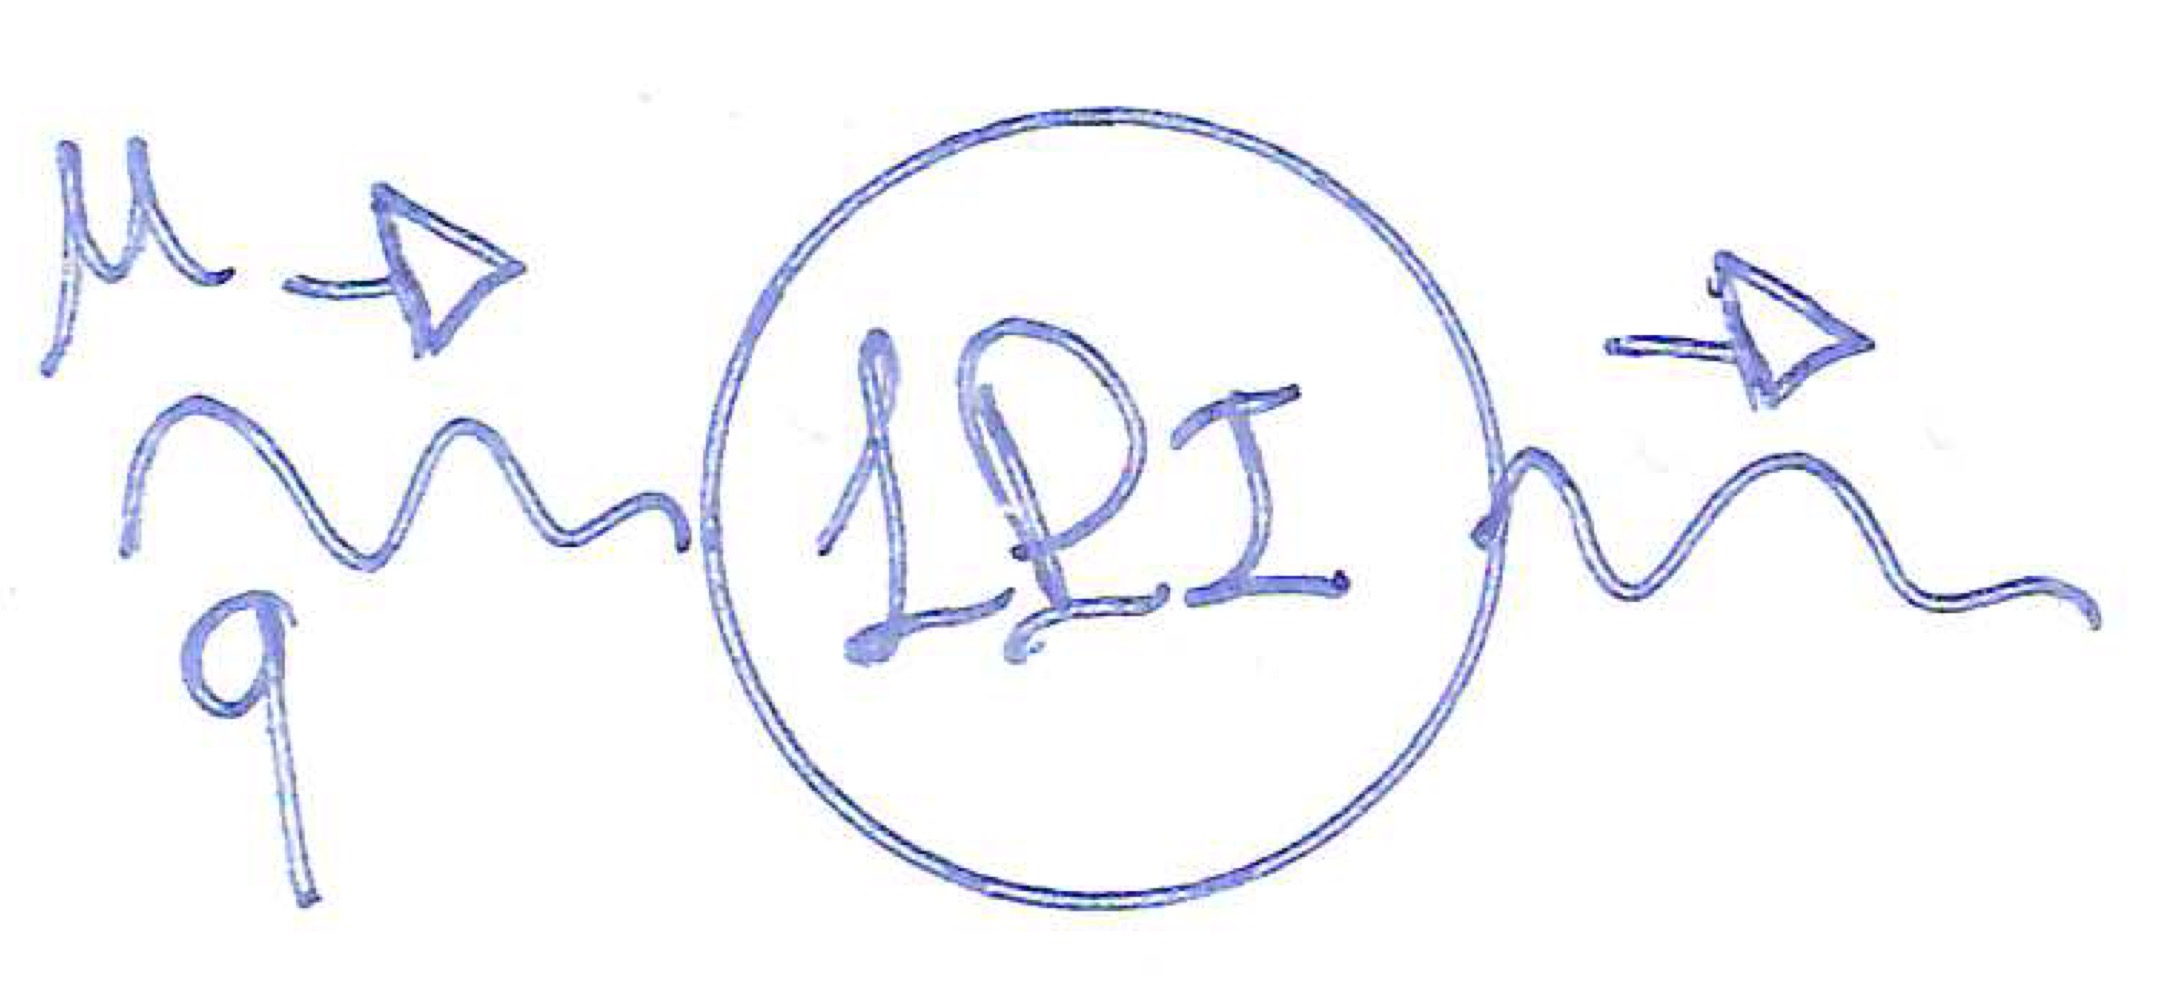
\includegraphics[]{images_ch2/photon_self_energy.JPG} 

Questo diagramma, per quanto visto nel capitolo \ref{ch:divergence}, ha un grado di divergenza superficiale pari a $D=4-\cancel{3/2N_e} - N_\gamma = 2$ e nel seguito adotteremo la notazione $\boxed{PSE \equiv i\Pi^{\mu\nu}(q)}$.

Partiamo da alcune considerazioni:
\begin{enumerate}
    \item \textbf{Covarianza di Lorentz.} \\
        $\Pi^{\mu\nu}(q)$ è un tensore di Lorentz costruito con $g^{\mu\nu}$ e $q^{\mu}$, quindi deve avere la struttura:
        \begin{equation}
            \Pi^{\mu\nu}(q) = \Theta(q^2)g^{\mu\nu} - \Pi(q^2)q^\mu q^\nu
            \label{eq:PSE_struct}
        \end{equation}
        Dove $\Theta(q^2)$ e $\Pi(q^2)$ sono funzioni scalari di $q^2=q^\mu q_\mu$.
        
    \item \textbf{Identità di Ward-Takahashi, $q_\mu\Pi^{\mu\nu}(q)=0$.} \\
        Per quanto appena visto otteniamo:
        \[
        q_\mu\Pi^{\mu\nu}(q)=\Theta(q^2)\underbrace{q_\mu g^{\mu\nu}}_{q_\nu} - \Pi(q^2)q^2 q^\nu = \underbrace{[\Theta(q^2) - \Pi(q^2)q^2]}_{\textcolor{Red}{{\Theta(q^2) = q^2\Pi(q^2)}}}q^\nu  \textcolor{Red}{\overset{!}{=} 0}
        \]
        di conseguenza, sostituendo nell'equazione (\ref{eq:PSE_struct}):
        \begin{equation}
            \Pi^{\mu\nu}(q) = (q^2g^{\mu\nu}-q^\mu q^\nu)\Pi(q^2)
            \label{eq:PSE_struct_revised}
        \end{equation}
        
    \item \textbf{Regolarità:} $i\Pi^{\mu\nu}$ non può avere un polo in $q^2=0$.\marginnote{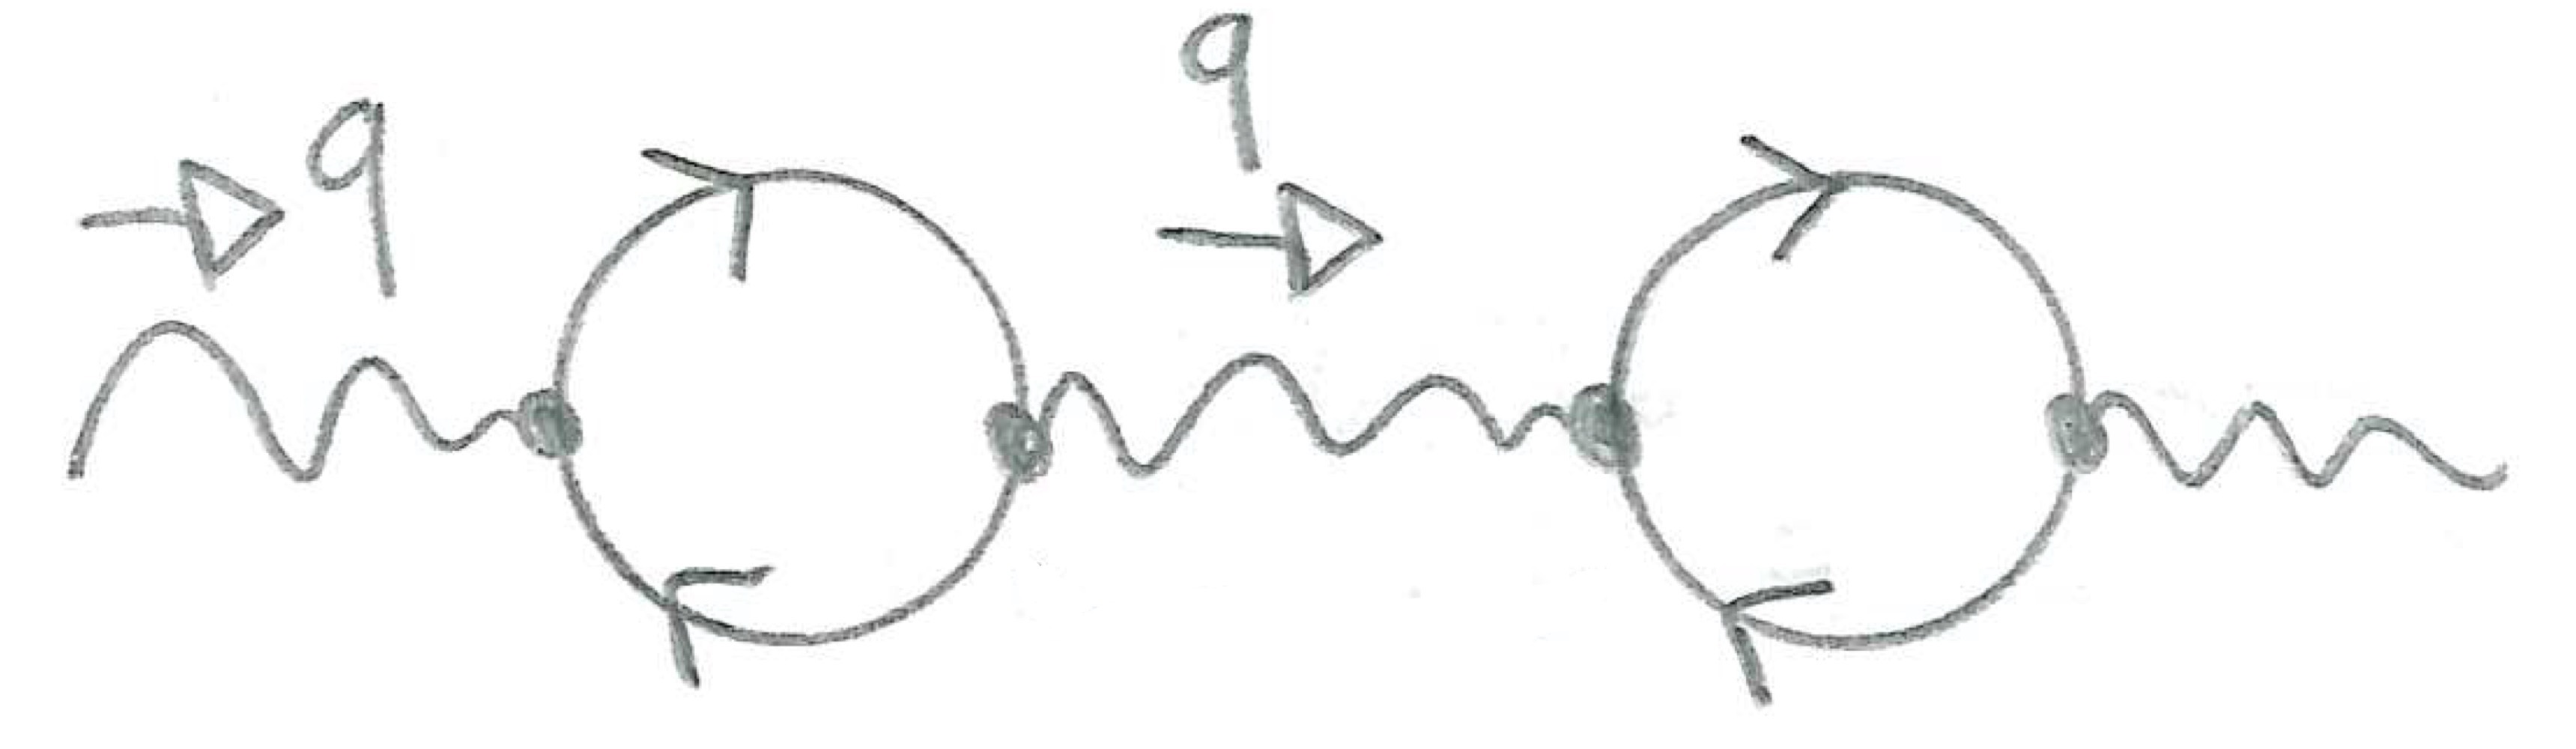
\includegraphics[]{images_ch2/PSE_polediag.jpg}} \\
        Un polo potrebbe apparire in un diagramma del tipo a lato, dove il propagatore intermedio porterebbe alla formazione del polo quando $q^2\rightarrow 0$, tuttavia questo diagramma non è 1PI\footnote{One-Particle Irreducible, nel senso espresso nella definizione \ref{def:1PI}} e non viene considerato nell'ampiezza da noi trattata.
\end{enumerate}

\begin{kaobox}
    Possiamo a questo punto riassumere quanto appena osservato:
    \begin{equation}
        \Pi^{\mu\nu}(q) = (q^2 g^{\mu\nu} - q^\mu q^\nu)\Pi(q^2)~ ~~ \Pi(q^2)\, \text{"regolare" per } q^2\rightarrow 0
        \label{eq:Pi_munu_summary}
    \end{equation}
\end{kaobox}

Consideriamo adesso un'espansione in serie di potenze di $\Pi^{\mu\nu}$ rispetto ad un 4-impulso esterno.

\begin{nota}
Di base il grado di divergenza della PSE è $D=2$. Come già discusso in precedenza, nella discussione attorno all'equazione (\ref{eq:amplit_powerseries}), derivare rispetto ad un impulso esterno corrisponde ad un decremento del grado di divergenza.
\end{nota}

Scriviamo quindi:

\begin{align*}
    \Pi^{\mu\nu}(q) =~ & \Pi^{\mu\nu}(q=0) + \tag*{\llap{(D=2)}} \\
                    & + \frac{\partial \Pi^{\mu\nu}}{\partial q^\rho}\bigg|_{q=0}q^\rho + \tag*{\llap{(D=1)}}\\
                    & + \frac{\partial^2 \Pi^{\mu\nu}}{\partial q^\rho\partial q^\sigma}\bigg|_{q=0}q^\rho q^\sigma + \frac{\partial^2 \Pi^{\mu\nu}}{\partial q^\rho\partial q^\sigma}\bigg|_{q=0}q^2 g^{\rho\sigma} +  \tag*{\llap{(D=0)}}\\
                    & + \Pi^{\mu\nu}_\text{FINITE}(q) \tag*{\llap{(D<0)}}
\end{align*}
Se compariamo l'espansione in serie con l'equazione (\ref{eq:Pi_munu_summary}) due cose risultano evidenti:
\begin{enumerate}
    \item[i.] I termini divergenti con grado di divergenza pari a $D=2,~1$ sono assenti.
    \item[ii.] Il grado di divergenza maggiore di $\Pi^{\mu\nu}(q)$ è $D=0$, una divergenza "$\log\Lambda$", se parliamo in termini di cutoff.
\end{enumerate}

Quindi il grado di divergenza dell'ampiezza di autoenergia del fotone è pari a $\boxed{D=0}$.

\section{Calcolo esplicito ad 1 loop}
\label{sec:1loop_pse_calc}

È giunto il momento di lanciarci in uno di quei calcoli che \textit{conviene fare almeno una volta nella vita}, ossia quello dell'auto-energia del fotone con un loop, anche detta \href{https://it.wikipedia.org/wiki/Polarizzazione_del_vuoto}{\textbf{}{polarizzazione del vuoto}}: una coppia $e^+e^-$ virtuale viene prodotta da un campo elettromagnetico di fondo, modificando la distribuzione di carica che ha generato il campo elettromagnetico iniziale.

Il diagramma, che indichiamo con $\boxed{i\Pi^{\mu\nu}_{\text{1-loop}}(q)}$ è quello riportato al lato.\marginnote{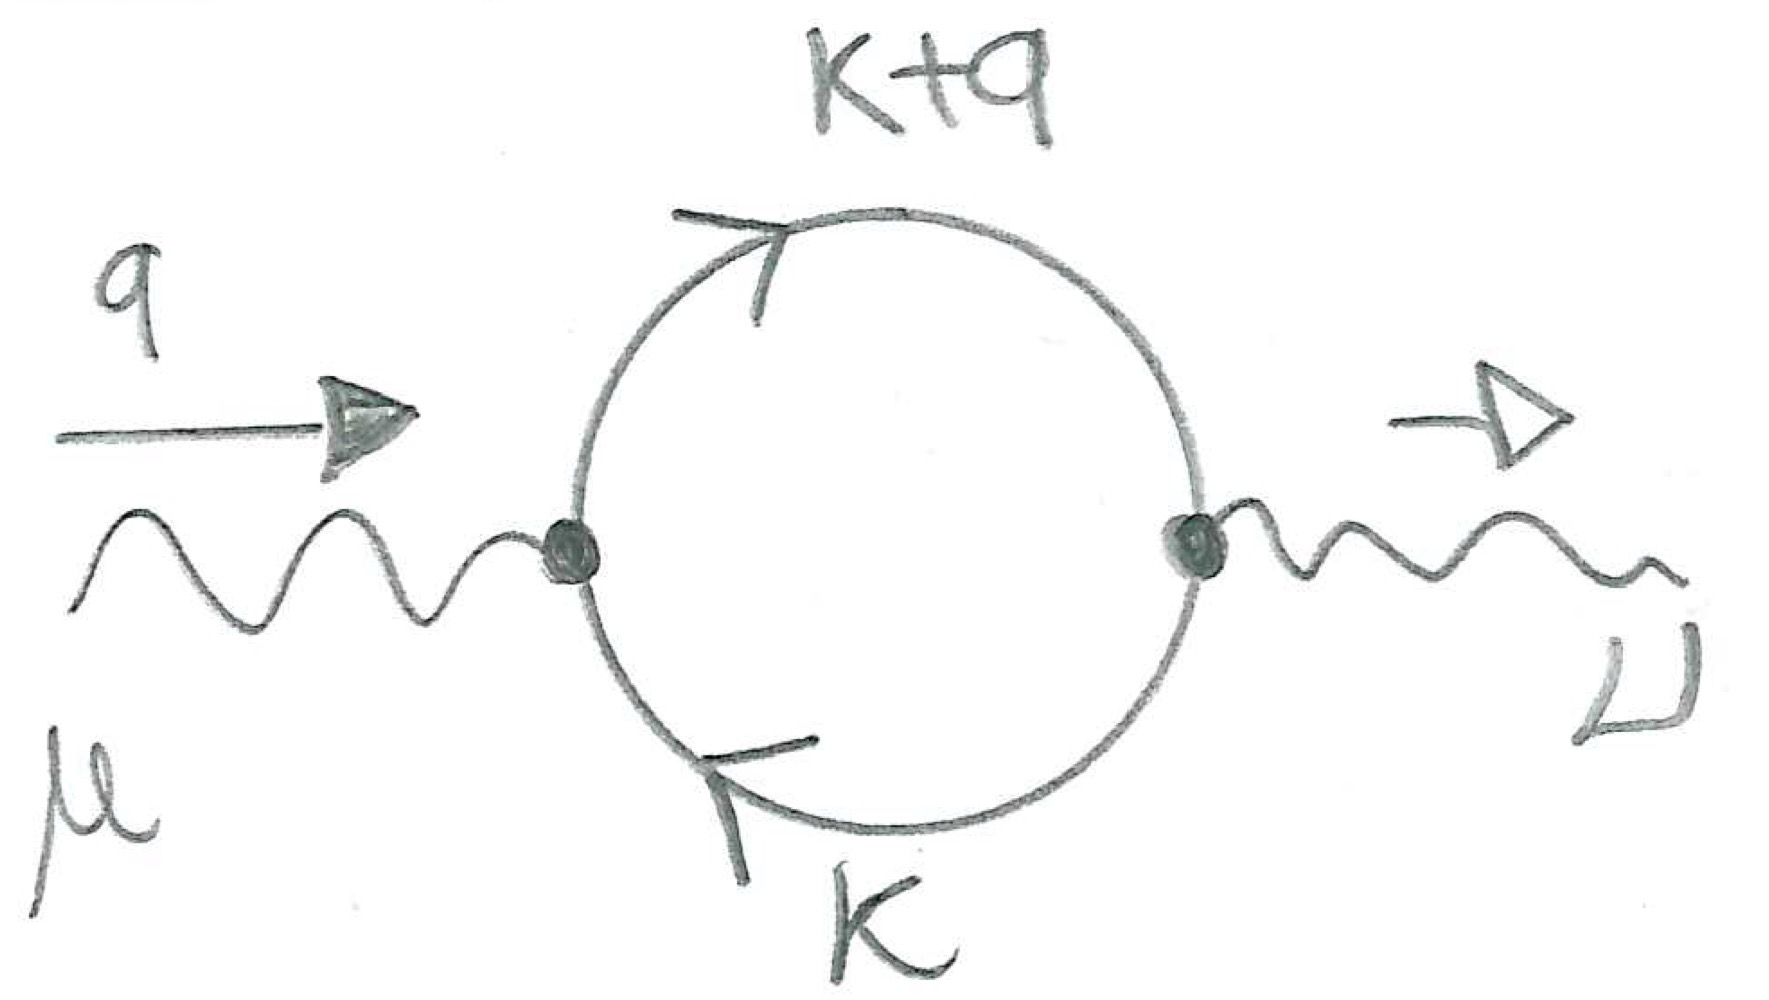
\includegraphics[]{images_ch2/PSE_1loop.jpg}\\ Diagramma di Feynman per la polarizzazione del vuoto.}

Con la notazione adottata, l'ampiezza del diagramma può essere scritta sulla base delle regole di Feynman, partendo dal vertice $\mu$ e andando in verso opposto rispetto alle linee fermioniche, come segue:

\begin{equation}
    i\Pi^{\mu\nu}_{\text{1-loop}}(q) = (-1)(ie)^2\int \frac{d^4k}{(2\pi)^4} \frac{\tr{\gamma^\mu i (\slashed k + m)\gamma^\nu i(\slashed k + \slashed q + m)}}{(k^2-m^2+i\varepsilon)\bigl[(k+q)^2-m^2+i\varepsilon\bigr]}
    \label{eq:PSE_1loop_feynman}
\end{equation}


\subsection{Regole generali}

Giustifichiamo l'equazione (\ref{eq:PSE_1loop_feynman}) in modo da dare una visione più concreta di quello che appare come un integrale mostruoso, questo ci consentirà anche di ricordare alcune regole utili ai fini della scrittura di integrali correlati a diagrammi di Feynman, oltre che introdurne di nuove nei casi che comprendono uno o più loop:
\begin{enumerate}
    \item $(ie)^2$ arriva dai due vertici di QED presenti nel diagramma, ogni vertice corrisponde ad un fattore $ie\gamma^\mu$.
    
    \item $(-1)$ è associato al loop chiuso di fermioni, ogni loop chiuso di fermioni porta con se un fattore (-1) in un diagramma a più di un loop. Il motivo di questo segno meno apparirà chiaro tra poco, nella nota \ref{note:wick_contraction}.
    
    \item $\int \frac{d^4k}{(2\pi)^4}$ deriva dal fatto che integriamo su ogni 4-impulso non vincolato da leggi di conservazione di 4-impulsi al vertice.
    
    \item Come già anticipato, la funzione integranda viene scritta partendo da un vertice generico, nel nostro caso dal vertice $\mu$, poi si va in verso opposto rispetto alle linee fermioniche, quindi si scrive il propagatore associato al positrone con 4-impulso $k$, poi il vertice $\nu$ e infine il propagatore dell'elettrone con 4-impulso $(k+q)$.
    
    \item La traccia al numeratore (che agisce sugli indici di Lorentz) deriva invece dalla somma sullo spin, necessaria in quanto le linee fermioniche sono chiuse.
\end{enumerate}
\begin{nota}
    \textbf{(Origine del $(-1)$ e di $\tr{\cdot\cdot\cdot}$)}\\
    Ricordiamo che il propagatore fermionico è dato dall'espressione:
    \begin{align*}
        i\bigl[S_F(x-y)\bigr]_{\alpha\beta} &= \overbrace{\langle0| T[\psi_\alpha(x)\bar{\psi}_\alpha(y)] |0\rangle}^{\textcolor{Red}{\text{"Contrazione di Wick"}}} \textcolor{Red}{\equiv \wick{\c1 {\psi}_\alpha(x) \c1{\bar{\psi}}_\beta(y) }}\\
                &= \int \frac{d^4p}{(2\pi)^4} e^{-ip\cdot(x-y)} \frac{i[\slashed p + m]_{\alpha\beta}}{p^2-m^2+i\varepsilon}
    \end{align*}
    Il punto cruciale è che \textbf{l'ordine degli operatori è importante}. In altre parole:
    \[
    \wick[wickcolor=black]{\c{\bar{\psi}}_\alpha(x) \c{\psi}_\beta(y)} = (-1)\wick[wickcolor=black]{\c{\psi}_\beta(y) \c{\bar{\psi}}_\alpha(x)} = (-1)i\bigr[S_F(y-x)\bigl]_{\beta\alpha}
    \]

    Di conseguenza, se consideriamo le varie contrazioni nell'elemento di matrice, siamo di fronte alla seguente situazione:
    \[
    \wick[positions={-1,+1,+1,-1}]{
        \langle \c1{A}(q) | (ie) \c2{\bar{\psi}}_\alpha(x)\bigl[\gamma^\mu\bigr]_{\alpha\beta} \c1{A}_\mu(x)\c3{\psi}_\beta(x) \, (ie) \c3{\bar{\psi}}_\rho(y)\bigl[\gamma^\nu\bigr]_{\rho\delta}\c4{A}_\nu(y)\c2{\psi}_\delta(y)  | \c4{A}(q) \rangle
    }
    \]
    Delle due contrazioni fermioniche, quella interna corrisponde al propagatore fermionico, quella esterna invece ha i campi invertiti, quindi porterà un fattore $(-1)$ globale, quello che troviamo nella (\ref{eq:PSE_1loop_feynman}).

    Esplicitando i propagatori troviamo:
    \[
    (ie)^2 \bigl[\gamma^\mu\bigr]_{\alpha\beta} i\bigl[S_F(x-y)\bigr]_{\beta\rho}  \, \bigl[\gamma^\nu\bigr]_{\rho\delta}(-1)i\bigl[S_F(y-x)\bigr]_{\delta\alpha}
    \]
    e sommando sugli spin chiudiamo la traccia! 
    \label{note:wick_contraction}
\end{nota}

\begin{nota}
    Va detto che di norma quando si trattano diagrammi come questi, assumendo impulso $q$ per le gambe esterne, l'elemento di matrice associato è qualcosa del tipo:
    \[
    i\mathscr{M} = \varepsilon_\mu(q)\varepsilon_\nu(q)i\Pi^{\mu\nu}(q)
    \]
    Tuttavia ci concentriamo sulla parte tensoriale, in modo da poter utilizzare i risultati così ottenuti anche nel caso in cui si consideri un diagramma più grande contenente una parte simil-PSE, in cui i fotoni esterni agiscono da propagatore.
    \label{note:polariz_neglect}
\end{nota}
\subsection{Svolgimento del calcolo}
Cominciamo con il calcolo esplicito e partiamo con le dovute semplificazioni del caso, sfruttando le proprietà delle matrici $\gamma$:
\marginnote{Ricordiamo che $\tr(n\gamma)=0$ quando $n$ è dispari.}
\begin{align*}
    i\Pi^{\mu\nu}_{\text{1-loop}}(q) &= (-1)(ie)^2\int \frac{d^4k}{(2\pi)^4} \frac{\tr{\gamma^\mu i (\slashed k + m)\gamma^\nu i(\slashed k + \slashed q + m)}}{(k^2-m^2+i\varepsilon)\bigl[(k+q)^2-m^2+i\varepsilon\bigr]} \\
    & = - e^2\int \frac{d^4k}{(2\pi)^4} \frac{ \overbrace{\tr{\gamma^\mu \slashed k \gamma^\nu (\slashed k + \slashed q)}}^{\textcolor{Red}{\tr{\gamma^\mu\gamma^\rho k_\rho\gamma^\nu\gamma^\sigma(k+q)_\sigma}} } + m^2\overbrace{\tr{\gamma^\mu\gamma^\nu}}^{\textcolor{Red}{=4g^{\mu\nu}}} }{(k^2-m^2+i\varepsilon)\bigl[(k+q)^2-m^2+i\varepsilon\bigr]}\\
    & = - \textcolor{Red}{4}e^2\int \frac{d^4k}{(2\pi)^4} \frac{ \textcolor{Red}{k^\rho(k + q)^\sigma (g^{\mu\rho}g^{\nu\sigma} - g^{\mu\nu}g^{\rho\sigma} + g^{\mu\sigma}g^{\nu\rho})} + m^2\textcolor{Red}{g^{\mu\nu}}}{(k^2-m^2+i\varepsilon)\bigl[(k+q)^2-m^2+i\varepsilon\bigr]} \\
    & = - 4e^2\int \frac{d^4k}{(2\pi)^4} \frac{ k^\mu(k + q)^\nu - k\cdot(k+q)g^{\mu\nu} + k^\nu(k + q)^\mu + m^2g^{\mu\nu}}{(k^2-m^2+i\varepsilon)\bigl[(k+q)^2-m^2+i\varepsilon\bigr]}
\end{align*}


Il primo risultato che otteniamo è quindi:
 \begin{equation}
    i\Pi^{\mu\nu}_{\text{1-loop}}(q) = - 4e^2\int \frac{d^4k}{(2\pi)^4} \frac{ k^\mu(k + q)^\nu + k^\nu(k + q)^\mu - g^{\mu\nu}\bigl[k\cdot(k+q) - m^2\bigr]}{(k^2-m^2+i\varepsilon)\bigl[(k+q)^2-m^2+i\varepsilon\bigr]} 
    \label{eq:Pi_munu_simplif_1}
 \end{equation}

\subsubsection{Introduciamo il parametro di Feynman}
L'idea è quella di utilizzare l'identità:
\begin{equation}
    \frac{1}{AB} = \int_0^1dx\frac{1}{\bigl[(1- x)A+xB\bigr]^2}
    \label{eq:feynman_formula}
\end{equation}
detta "formula di Feynman", dove $x$ è detto \textit{parametro di Feynman}, prendendo 
\begin{align*}
A &\equiv (k^2-m^2+i\varepsilon) \\
B &\equiv (k+q)^2 - m^2 +i\varepsilon
\end{align*}
\begin{exercise}
Dimostrare l'identità (\ref{eq:feynman_formula}) [\textbf{svolto lezione 4 p.8÷9}]
\end{exercise}

\subsubsection{Applichiamo la formula di Feynman}
Lavoriamo sul denominatore dell'integrale (\ref{eq:feynman_formula}), sostituendo $A$ e $B$ come detto sopra, con della banale algebra si trova:
\begin{align*}
\text{den} & = \Bigl\{ (1-x)(k^2-m^2+i\varepsilon) + x\bigl[(k+q)^2 - m^2 +i\varepsilon\bigr] \Bigr\}^2 \\
    & = \bigl[(k+xq)^2 + xq^2(1-x) - m^2 + i\varepsilon \bigr]^2 
\end{align*}

Otteniamo quindi un secondo risultato:
\begin{equation}
    \frac{1}{(k^2-m^2+i\varepsilon)\bigl[(k+q)^2 - m^2 +i\varepsilon\bigr]} = \int_0^1dx\frac{1}{\bigl[(k+xq)^2 + xq^2(1-x) - m^2 + i\varepsilon\bigr]^2}
    \label{eq:feynm_applic}
\end{equation}

\subsubsection{Torniamo all'integrale al loop}

Combinando la (\ref{eq:Pi_munu_simplif_1}) con la (\ref{eq:feynm_applic}) otteniamo:
\begin{equation}
    i\Pi^{\mu\nu}_{\text{1-loop}}(q) = - 4e^2\int \frac{d^4k}{(2\pi)^4}\int_0^1dx \frac{ k^\mu(k + q)^\nu + k^\nu(k + q)^\mu - g^{\mu\nu}\bigl[k\cdot(k+q) - m^2\bigr]}{\bigl[(k+xq)^2 + xq^2(1-x) - m^2 + i\varepsilon\bigr]^2} 
    \label{eq:Pi_munu_simplif_2}
\end{equation}

Saremmo adesso tentati dall'invertire gli integrali, cambiando anche la variabile di integrazione in $l\equiv k+xq$; tuttavia ciò sarebbe possibile solo nel caso in cui l'integrale in $k$ converga, e non è questo il caso!

\subsubsection{Regolarizzazione dimensionale}
Prima di procedere con il calcolo dobbiamo quindi \textit{regolarizzare la teoria}: dobbiamo “deformarla” in modo tale da rendere l'integrale in $k$ convergente.

Per fare ciò \textbf{riduciamo il numero di dimensioni spazio-temporali ($4\rightarrow\mathsf d < 4$)}, questo step è noto come \textit{Regolarizzazione Dimensionale}, o \textbf{DIMREG}.

Alla fine dei conti, torneremo in 4 dimensioni e apparirà nuovamente la divergenza che abbiamo nascosto sotto al tappeto, ma quello che la DIMREG ci permette di fare è isolare in modo chiaro la parte divergente dell'integrale.

Riscriviamo allora nuovamente la (\ref{eq:Pi_munu_simplif_2}), cambiando la variabile di integrazione in $l^\mu\equiv k^\mu+xq^\mu$, definendo $\boxed{\Delta \equiv m^2 - x(1-x)q^2}$ ed applicando la DIMREG (che ci permette di invertire l'ordine di integrazione):

\begin{equation}
    \boxed{
    i\Pi^{\mu\nu}_{\text{1-loop}}(q) = - 4e^2\int_0^1dx \int \frac{d^\mathsf{d} l}{(2\pi)^\mathsf{d}} \frac{ \mathscr{N^{\mu\nu}}}{(l^2 - \Delta + i\varepsilon)^2}
    }
    \label{eq:Pi_munu_simplif_3}
\end{equation}

dove il numeratore, sostituendo $k^\mu\equiv l^\mu - xq^\mu$, assume la forma:

\begin{align*}
    \mathscr{N}^{\mu\nu}= &~  l^\mu l^\nu + l^\mu+(1-x)q^\nu - xq^\mu l^\nu - xq^\mu(1-x)q^\nu + \\
                         & + l^\nu l^\mu + l^\nu+(1-x)q^\mu - xq^\nu l^\mu - xq^\nu(1-x)q^\mu + \\
                         & - g^{\mu\nu}[l^2 + l\cdot q+(1-x) - xq\cdot l - x(1-x)q^2 - m^2] \\
\end{align*}

Tuttavia, per la struttura dell'integrale, c'è da considerare il fatto che gli integrali dei termini lineari in $l^\mu$ andranno a zero per ragioni di parità ($l^\mu\rightarrow - l^\mu$).
Di conseguenza:

\begin{equation}
    \mathscr{N}^{\mu\nu} \xrightarrow[\text{lineari in } l^\mu]{\text{senza termini}} 2l^\mu l^\nu - g^{\mu\nu}l^2 - 2x(1-x)q^\mu q^\nu + g^{\mu\nu}[m^2 + x(1-x)q^2]
    \label{eq:numerator_no_lin_terms}
\end{equation}

\subsubsection{Riduzione delle strutture tensoriali}

Se scorporiamo l'integrale (\ref{eq:Pi_munu_simplif_3}) in somme di più integrali (uno per ciascun termine del numeratore) e guardiamo il primo, tralasciando l'integrazione in $dx$, abbiamo a che fare con un integrale tensoriale. L'argomento di questo integrale è però solo funzione di $\Delta$, che è una quantità scalare.

Ci aspettiamo allora come risultato:

\[
\int \frac{d^\mathsf{d} l}{(2\pi)^\mathsf{d}} \frac{l^\mu l^\nu}{(l^2 - \Delta + i\varepsilon)^2} = \mathscr{I}(\Delta)g^{\mu\nu}
\]

con $g^{\mu\nu}$ a tener conto della struttura tensoriale.

Possiamo quindi risolvere per $\mathscr{I}(\Delta)$, moltiplicando ambo i lati per $g_{\mu\nu}$ e ricordando che $g_{\mu\nu}g^{\mu\nu}=\mathsf d$:

\[
\mathscr{I}(\Delta) = \int \frac{d^\mathsf{d} l}{(2\pi)^\mathsf{d}} \frac{l^2/\mathsf d}{(l^2 - \Delta + i\varepsilon)^2}
\]

Sostituendo nell'espressione sopra troviamo quindi:

\begin{equation}
    \boxed{\int \frac{d^\mathsf{d} l}{(2\pi)^\mathsf{d}} \frac{l^\mu l^\nu}{(l^2 - \Delta + i\varepsilon)^2} = \int \frac{d^\mathsf{d} l}{(2\pi)^\mathsf{d}} \frac{{g^{\mu\nu}l^2}/\mathsf d}{(l^2 - \Delta + i\varepsilon)^2}}
    \label{eq:tensor_reduction}
\end{equation}

Quanto appena visto ci permette di accorpare i primi due termini della (\ref{eq:numerator_no_lin_terms}) che quindi diventa:

\begin{equation}
    \mathscr{N}^{\mu\nu} = -(1 - \nicefrac{2}{\mathsf d}) l^2g^{\mu\nu} - 2x(1-x)q^\mu q^\nu + [m^2 + x(1-x)q^2] g^{\mu\nu}
    \label{eq:numerator_tensor_red}
\end{equation}

\subsubsection{Effettuiamo una rotazione di Wick}
Tralasciando la descrizione nel dettaglio di cosa una rotazione di Wick sia [\textbf{Lezione 5 p.13÷15}], quello che ci interessa fare è semplificare il calcolo dell'integrale in (\ref{eq:Pi_munu_simplif_3}), per farlo "ruotiamo una parte della funzione integranda di ${\pi}/{2}$", introducendo un tempo immaginario.

In termini matematici, ad una rotazione di Wick corrisponde la sostituzione $\boxed{l^0\rightarrow il^0_E}$, con $l^0_E\in(-\infty,+\infty)$ e dove $l^0$ è la componente 0 ("temporale", se la pensiamo nella notazione dei 4-vettori) del $\mathsf d$-vettore $l = (l^0,\,l^1\,,...\,,l^\mathsf d ) = (l^0,\,\Vec{l} ) \Rightarrow l^2=({l^0})^2-|\Vec{l}|^2$.

\begin{nota}
    \textbf{(Condizioni necessarie all'applicazione della rotazione di Wick)}
    È cruciale che l'integrale originale converga, in modo tale da poter trascurare l'integrale sugli archi nel cammino che si sceglie per evitare i poli della funzione. Di conseguenza è cruciale che venga effettuata prima la DIMREG, e poi la rotazione di Wick.

    Inoltre, in questa discussione stiamo assumendo che $\Delta$ sia una quantità positiva. Vedremo invece che, studiando il teorema ottico in sezione \ref{sec:opt_theorem}, sarà cruciale considerare il caso in cui $\Delta<0$.
\end{nota}
\marginnote{È degno di nota il fatto che, spostando l'integrazione sull'asse immaginario evitando i poli, ci troviamo nella situazione in cui possiamo permetterci di trascurare il fattore $i\varepsilon$ al denominatore, questo è schematizzabile nello sketch qui sotto, in cui $\lambda_2$ è parametrizzato da $l^0=il^0_E$.\\
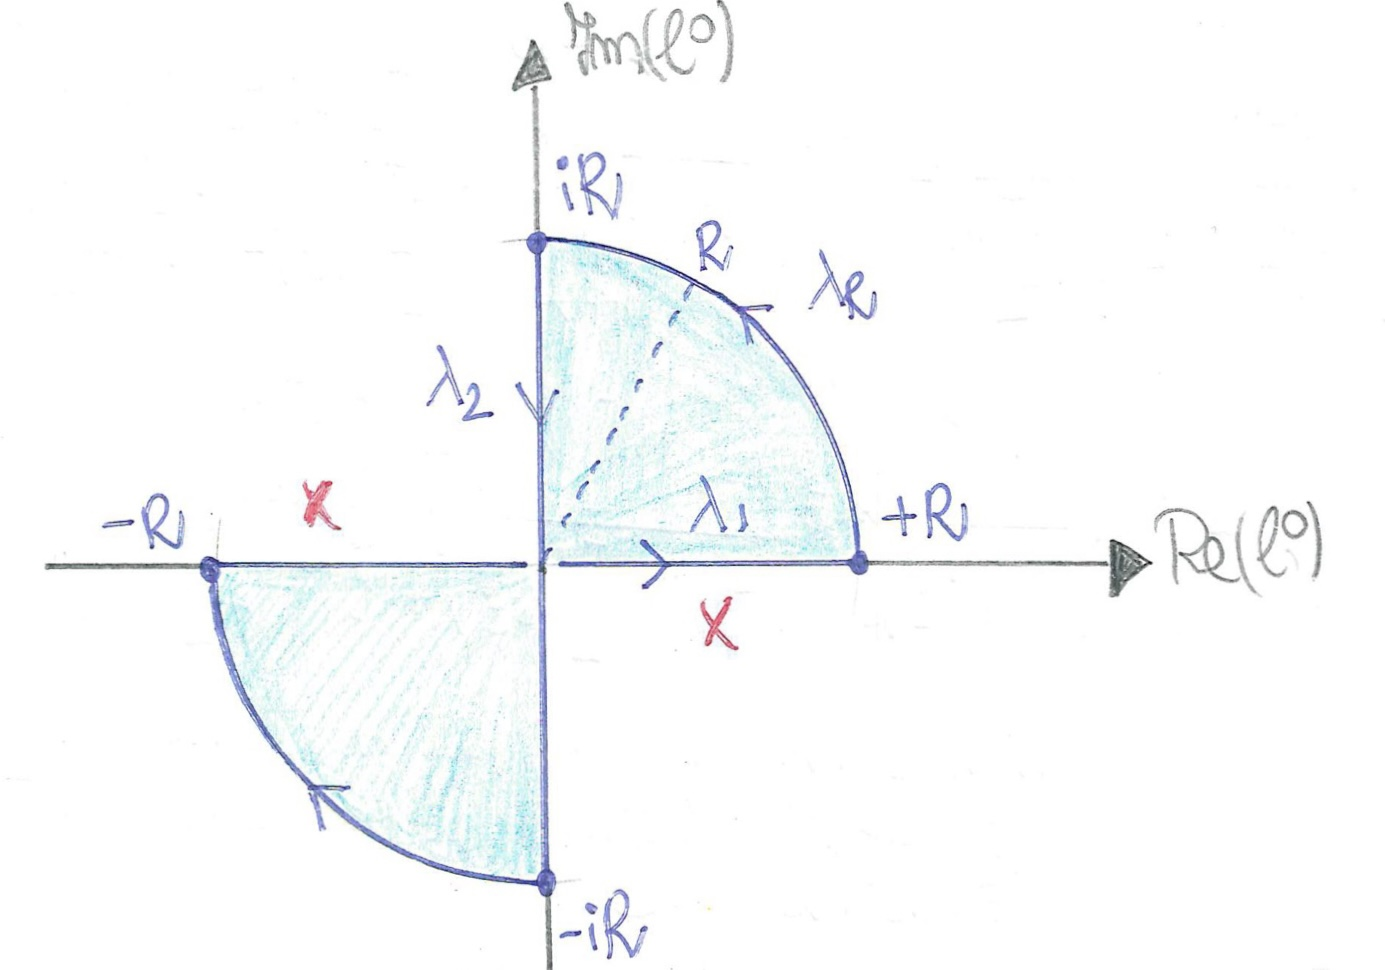
\includegraphics[]{images_ch2/wick-rotation.jpg}

Inoltre notiamo, come riportato in equazione (\ref{eq:Pi_munu_rotated}), solo il primo termine del numeratore cambia di segno, grazie al $(-1)^{n-m} = (-1)^{-1} = -1$.
}

Introducendo quindi il vettore Euclideo $\mathsf d$-dimensionale $\Vec{l_E}=(l^0_E,\Vec{l})$, tale per cui $|\Vec{l_E}|^2 = ({l^0_E})^2 + |\Vec{l}|^2$ (con il $+$ !), la rotazione di Wick si esprime nella sua forma generale come segue (notare il cambio di segno di $\Delta$):

\begin{equation}
    \boxed{
    \int \frac{d^\mathsf{d} l}{(2\pi)^\mathsf{d}} \frac{l^{2n}}{(l^2 - \Delta + i\varepsilon)^m} = (-1)^{n-m} i \int \frac{d^\mathsf{d} \Vec{l_E}}{(2\pi)^\mathsf{d}} \frac{|\Vec{l_E}|^{2n}}{\bigl[|\Vec{l_E}|^2 + \Delta\bigr]^m}
    }
    \label{eq:wick_rotation}
\end{equation}

Applichiamo ora la (\ref{eq:wick_rotation}) alla (\ref{eq:Pi_munu_simplif_3}), che corrisponde al caso con $n=1$ ed $m=2$, sostituendo anche il numeratore come scritto nella (\ref{eq:numerator_tensor_red}) e otteniamo:

\begin{equation}
    \boxed{
    \begin{aligned}
        &i\Pi^{\mu\nu}_{\text{1-loop}}(q)  = - 4ie^2\int_0^1dx \int \frac{d^\mathsf{d} \Vec{l_E}}{(2\pi)^\mathsf{d}} \frac{ \mathscr{N}^{\mu\nu}_E }{\bigl[|\Vec{l_E}|^2 + \Delta\bigr]^2} \\
        \mathscr{N}^{\mu\nu}_E & = (1 - \nicefrac{2}{\mathsf d}) |\Vec{l_E}|^2g^{\mu\nu} - 2x(1-x)q^\mu q^\nu + [m^2 + x(1-x)q^2]g^{\mu\nu}
    \end{aligned}}
    \label{eq:Pi_munu_rotated}
\end{equation}

\subsubsection{Svolgiamo l'integrale Euclideo}
Più facile a dirsi che a farsi, ci sono un bel po' di conti da fare [\textbf{Lez 5 p.17÷22}].

Quello che ci interessa portare a casa è che introducendo le coordinate polari $\mathsf d$-dimensionali, separando l'integrale nelle sue componenti radiali e angolari e sfruttando alcuni integrali notevoli, si può scrivere nel caso più generale:

\begin{equation}
    \int \frac{d^\mathsf{d} \Vec{l_E}}{(2\pi)^\mathsf{d}} \frac{\bigl(|\Vec{l_E}|^2\bigr)^n}{\bigl[|\Vec{l_E}|^2 + \Delta\bigr]^m} = \frac{1}{(4\pi)^{\nicefrac{\mathsf d}{2}}} \bigg(\frac{1}{\Delta}\bigg)^{m-n-\nicefrac{\mathsf d}{2}}\frac{\Gamma(m-n-\nicefrac{\mathsf d}{2})\Gamma(n+\nicefrac{\mathsf d}{2})}{\Gamma(\nicefrac{\mathsf d}{2})\Gamma(m)}
    \label{eq:euclidean_integral_general}
\end{equation}


A noi interessano due casi specifici:
\begin{enumerate}
    \item ($n=0$, $m=2$) Da cui si ottiene:
        \begin{equation}
            \int \frac{d^\mathsf{d} \Vec{l_E}}{(2\pi)^\mathsf{d}} \frac{1}{\bigl[|\Vec{l_E}|^2 + \Delta\bigr]^2} = \frac{1}{(4\pi)^{\nicefrac{\mathsf d}{2}}} \frac{\Gamma(2-\nicefrac{\mathsf d}{2})}{\Gamma(2)}\bigg(\frac{1}{\Delta}\bigg)^{2-\nicefrac{\mathsf d}{2}}
            \label{eq:euclidean_integral_n0m2}
        \end{equation}
    
    \item ($n=1$, $m=2$) Da cui otteniamo:
        \begin{equation}
            \int \frac{d^\mathsf{d} \Vec{l_E}}{(2\pi)^\mathsf{d}} \frac{|\Vec{l_E}|^2}{\bigl[|\Vec{l_E}|^2 + \Delta\bigr]^2} = \frac{1}{(4\pi)^{\nicefrac{\mathsf d}{2}}} \frac{\Gamma(2-\nicefrac{\mathsf d}{2})}{\Gamma(2)}\bigg(\frac{1}{\Delta}\bigg)^{2-\nicefrac{\mathsf d}{2}} \frac{d}{2} \frac{\Delta}{(1-\nicefrac{\mathsf d}{2})}
            \label{eq:euclidean_integral_n1m2}
        \end{equation}
        usando in maniera opportuna alcune identità delle $\Gamma$ di Eulero in modo ottenere una struttura simile a quella nel caso 1. 
\end{enumerate} 

Applichiamo allora queste formule al nostro integrale, in cui abbiamo un integrale di tipo 2. e due integrali di tipo 1. (corrispondenti rispettivamente al primo e ai successivi termini presenti nel numeratore).

Otteniamo, sfruttando il fatto che $\Gamma(2)=1$:

\begin{align*}
    i\Pi^{\mu\nu}_{\text{1-loop}}(q)  = & - 4ie^2\int_0^1dx \frac{1}{(4\pi)^{\nicefrac{\mathsf d}{2}}} \frac{\Gamma(2-\nicefrac{\mathsf d}{2})}{\Gamma(2)} \times \bigg\{ (1 - \nicefrac{2}{\mathsf d})g^{\mu\nu} \frac{d}{2}\frac{\Delta}{(1 - \nicefrac{\mathsf d}{2})} + \\
    &+ [-2x(1-x)q^\mu q^\nu + m^2g^{\mu\nu}+x(1-x)q^2g^{\mu\nu}]\bigg\} \overset{\star}{=}
\end{align*}

La cosa interessante, oserei dire fantastica, è che se operiamo le giuste sostituzioni nella parte tra le parentesi graffe avvengono delle magiche semplificazioni e alla fine dei conti:

\begin{align*}
    \overset{\star}{=} - 4ie^2\int_0^1dx \frac{1}{(4\pi)^{\nicefrac{\mathsf d}{2}}} \frac{\Gamma(2-\nicefrac{\mathsf d}{2})}{\Gamma(2)} 2x(1-x)(q^2g^{\mu\nu}-q^\mu q^\nu)
\end{align*}

Che al lettore più attento potrebbe sembrare familiare\footnote{se così non fosse, si confronti con la (\ref{eq:PSE_struct_revised})}.


In sintesi:
\begin{equation}
    \begin{aligned}
        &i\Pi^{\mu\nu}_{\text{1-loop}}(q) = (q^2g^{\mu\nu}-q^\mu q^\nu) i \Pi_{\text{1-loop}}(q^2) \\
        &\Pi_{\text{1-loop}}(q^2) = \frac{-8e^2}{ (4\pi)^{\nicefrac{\mathsf d}{2}} } \int_0^1 dx\, x(1-x)\frac{\Gamma(2-\nicefrac{\mathsf d}{2})}{\Delta^{2-\nicefrac{\mathsf d}{2}}} \\
        &\text{con } \Delta \equiv m^2 - x(1-x)q^2
    \end{aligned}
    \label{eq:Pi_munu_summary_2}
\end{equation}

Fermiamoci ora per commentare quanto riportato in (\ref{eq:Pi_munu_summary_2}):
\begin{itemize}
    \item La struttura di $i\Pi^{\mu\nu}_{\text{1-loop}}(q)$ riflette quella che abbiamo tirato fuori dal cappello fin dall'inizio, riportata in (\ref{eq:PSE_struct_revised}): la struttura tensoriale viene fattorizzata.
    Questa è una caratteristica speciale della regolarizzazione dimensionale, per indicarla si dice che "\textbf{la DIMREG è compatibile con l'invarianza di gauge (nella forma delle identità di Ward-Takahashi)}".
    \item L'espressione di $i\Pi^{\mu\nu}_{\text{1-loop}}(q)$ è ancora valida nella teoria "deformata" in $\mathsf d$-dimensioni. Ricordiamo poi che la funzione $\Gamma(z)$ ha poli semplici per $z = 0,-1,-2,...$, quindi nella nostra espressione, la divergenza (UV) si manifesta nel limite $\mathsf d \rightarrow 4 \Rightarrow \Gamma(z=0)$
    \item D'altra parte, per $z>0$ la funzione $\Gamma(z)$ è perfettamente regolare, il che si riflette nella regolarità di $i\Pi^{\mu\nu}_{\text{1-loop}}(q)$ per $2-\mathsf d/2>0 \Rightarrow \mathsf d < 4$, come atteso.
    \item Ricordiamo che la funzione $\Gamma(z)$:
        \begin{itemize}
            \item Coincide con la funzione fattoriale quando trattata su $\mathbb{N}^+$.
            \item Può essere definita $\forall z\in\mathbb{C} : \Re{z}>0$ per mezzo della formula integrale $\Gamma(z)=\int_0^\infty e^{-t}t^{z-1}dt$.
            \item Ammette prolungamento analitico sull'insieme $\mathbb{C}\setminus\{ 0,-1,-2,...\}$.
        \end{itemize}
\end{itemize}

\subsubsection{Passaggio a dimensione continua}

Nella nostra espressione finale (\ref{eq:Pi_munu_summary_2}), la dimensione $\mathsf d$ della teoria risulta essere argomento della funzione $\Gamma$, tuttavia nessuno ci obbliga a considerarla come una variabile discreta!

Considerando quindi $\mathsf d$ come continua, rimodelliamo il limite $\mathsf d \rightarrow 4$ definendo: 
\[
\mathsf d \equiv 4 - 2\epsilon \Rightarrow \epsilon \equiv 2 - \frac{\mathsf d}{2}
\]
Espandendo ora $\Gamma(z)$ in serie di Laurent intorno al suo polo in $z=0$ otteniamo come risultato:
\begin{equation}
\Gamma\bigl(2 - \frac{\mathsf d}{2}\bigr) = \Gamma(\epsilon) = \frac{1}{\epsilon}-\mathbb{\gamma}+\mathscr O(\epsilon)
\label{eq:gamma_expansion}
\end{equation}
dove $\mathbb{\gamma}\simeq0.577$ è la costante di Eulero-Mascheroni.

Allo stesso tempo possiamo riscrivere:
\[
\frac{1}{(4\pi)^{\nicefrac{\mathsf d}{2}}}\bigg(\frac{1}{\Delta}\bigg)^{ 2 - \frac{\mathsf d}{2}} = \frac{1}{(4\pi)^{2}}\bigg(\frac{4\pi}{\Delta}\bigg)^{ \epsilon} 
\]
Utilizziamo a questo punto l'espansione $(a)^\epsilon = 1+\epsilon\log{a} + \mathscr{O}(\epsilon^2)$ la formula finale sarà:

\begin{equation}
    \frac{1}{(4\pi)^{\nicefrac{\mathsf d}{2}}}\bigg(\frac{1}{\Delta}\bigg)^{ 2 - \frac{\mathsf d}{2}} = \frac{1}{(4\pi)^{2}}\bigg[1 + \epsilon\log{\frac{4\pi}{\Delta}} + \mathscr{O}(\epsilon^2) \bigg]
    \label{eq:mult_factor_expansion}
\end{equation}

Non resta altro che applicare la (\ref{eq:gamma_expansion}) e la (\ref{eq:mult_factor_expansion}) alla (\ref{eq:Pi_munu_summary_2}); quello che otteniamo da queste sostituzioni, lasciando da parte i termini di $\mathscr{O}(\epsilon)$ e superiori, che vanno a zero quando $\epsilon\rightarrow0$ è:
\begin{equation}
    \Pi_{\text{1-loop}}(q^2) = \frac{-8e^2}{ (4\pi)^2 } \int_0^1 dx\,x(1-x)\bigg[\frac{1}{\epsilon} - \mathbb{\gamma} + \log{\frac{4\pi}{\Delta}}\bigg]
    \label{eq:scalar_Pi_munu_expanded}
\end{equation}
Osserviamo come \textbf{la divergenza UV si manifesta come un polo semplice quando $\mathbf{\epsilon\rightarrow0}$}

\subsubsection{Scala di rinormalizzazione}

\underline{\textbf{Attenzione}}: qualcuno a questo punto potrebbe tirare un sospiro di sollievo, pensando di aver finalmente raggiunto il risultato finale, tuttavia non è così. 

Infatti, se osserviamo bene il termine logaritmico, ricordando che $\Delta = m^2-x(1-x)q^2$ è una quantità non adimensionale (a.k.a. "\textbf{dimensionful}"\footnote{ndr.: nel seguito adotterò questo termine nel caso sia necessario specificare la non-adimensionalità di una certa quantità, in quanto non ritengo esista una traduzione abbastanza fedele da adottare.}), ne deduciamo che debba esserci un fattore mancante per fare in modo che l'argomento del logaritmo sia adimensionale ("\textbf{dimensionless}").

La sottigliezza da adottare per risolvere questo problema risiede nella dimensione di massa del coupling di QED, che ricordiamo essere:
\[
[e] = [M]^{2-\nicefrac{\mathsf d}{2}} \xrightarrow[\epsilon = 2-\nicefrac{\mathsf d}{2}]{} [e] = [M]^\epsilon
\]

Quello che notiamo è che il coupling è dimensionless per $\mathsf d = 4$, ma dimensionful per $\mathsf d \neq 4$.

Operiamo allora un \textit{rescaling del coupling elettromagnetico} quando passiamo in dimensione generica, in modo da mantenere il il coupling adimensionale qualunque sia la dimensione: $\boxed{e\rightarrow e\mu^\epsilon}$, dove $\mu$ è detto "\textbf{scala di rinormalizzazione}" ed è una scala di massa arbitraria.

Questo rescaling risolve il problema che abbiamo notato poco fa. Infatti nell'espressione di $\Pi_{\text{1-loop}}(q^2)$ figura un $e^2 \rightarrow e^2\mu^{2\epsilon}$ e noi non facciamo altro se non prendere il fattore $\mu^{2\epsilon}$ e integrarlo nell'espansione (\ref{eq:mult_factor_expansion}), ottenendo:

\begin{equation}
    \frac{\mu^{2\epsilon}}{(4\pi)^{\nicefrac{\mathsf d}{2}}}\bigg(\frac{1}{\Delta}\bigg)^{ 2 - \frac{\mathsf d}{2}} = \frac{1}{(4\pi)^2}\bigg(\frac{4\pi\mu^2}{\Delta}\bigg)^\epsilon = \frac{1}{(4\pi)^{2}}\bigg[1 + \epsilon\log{\frac{4\pi\mu^2}{\Delta}} + \mathscr{O}(\epsilon^2) \bigg]
    \label{eq:mult_factor_expansion_dimensionless}
\end{equation}

L'argomento del logaritmo è ora dimensionless e possiamo (finalmente!) scrivere il tanto agognato \textbf{risultato finale per l'auto-energia del fotone regolarizzata ad 1 loop}:

\begin{equation}
    \boxed{
    \begin{aligned}
        &i\Pi^{\mu\nu}_{\text{1-loop}}(q) = (q^2g^{\mu\nu}-q^\mu q^\nu) i \Pi_{\text{1-loop}}(q^2) \\
        & \Pi_{\text{1-loop}}(q^2) = \frac{-8e^2}{ (4\pi)^2 } \int_0^1 dx\,x(1-x)\bigg[\frac{1}{\epsilon} - \mathbb{\gamma} + \log{\frac{4\pi\mu^2}{\Delta}}\bigg] \\
        &\text{con } \Delta \equiv m^2 - x(1-x)q^2
    \end{aligned}
    }
    \label{eq:Pi_munu_summary_final}
\end{equation}

\section{L'auto-energia dell'elettrone}
Dopo aver visto il caso del fotone, passiamo ad analizzare un'altra ampiezza divergente: quella che rappresenta l'auto-energia dell'elettrone (\textbf{ESE}), con grado di divergenza $D=1$ e che indichiamo con $\boxed{i\bigl[\Sigma(p)\bigr]_{\alpha\beta}}$.
\marginnote{\textbf{Nota:} Gli indici $\alpha$ e $\beta$ si riferiscono alla natura matriciale di $\bigl[\Sigma(p)\bigr]_{\alpha\beta}$ (è in genere una matrice $4\times4$, per la precisione). Nel seguito, tuttavia, questi indici saranno lasciati sottintesi ed eventualmente esplicitati solo quando il contesto dovesse richiederlo.}

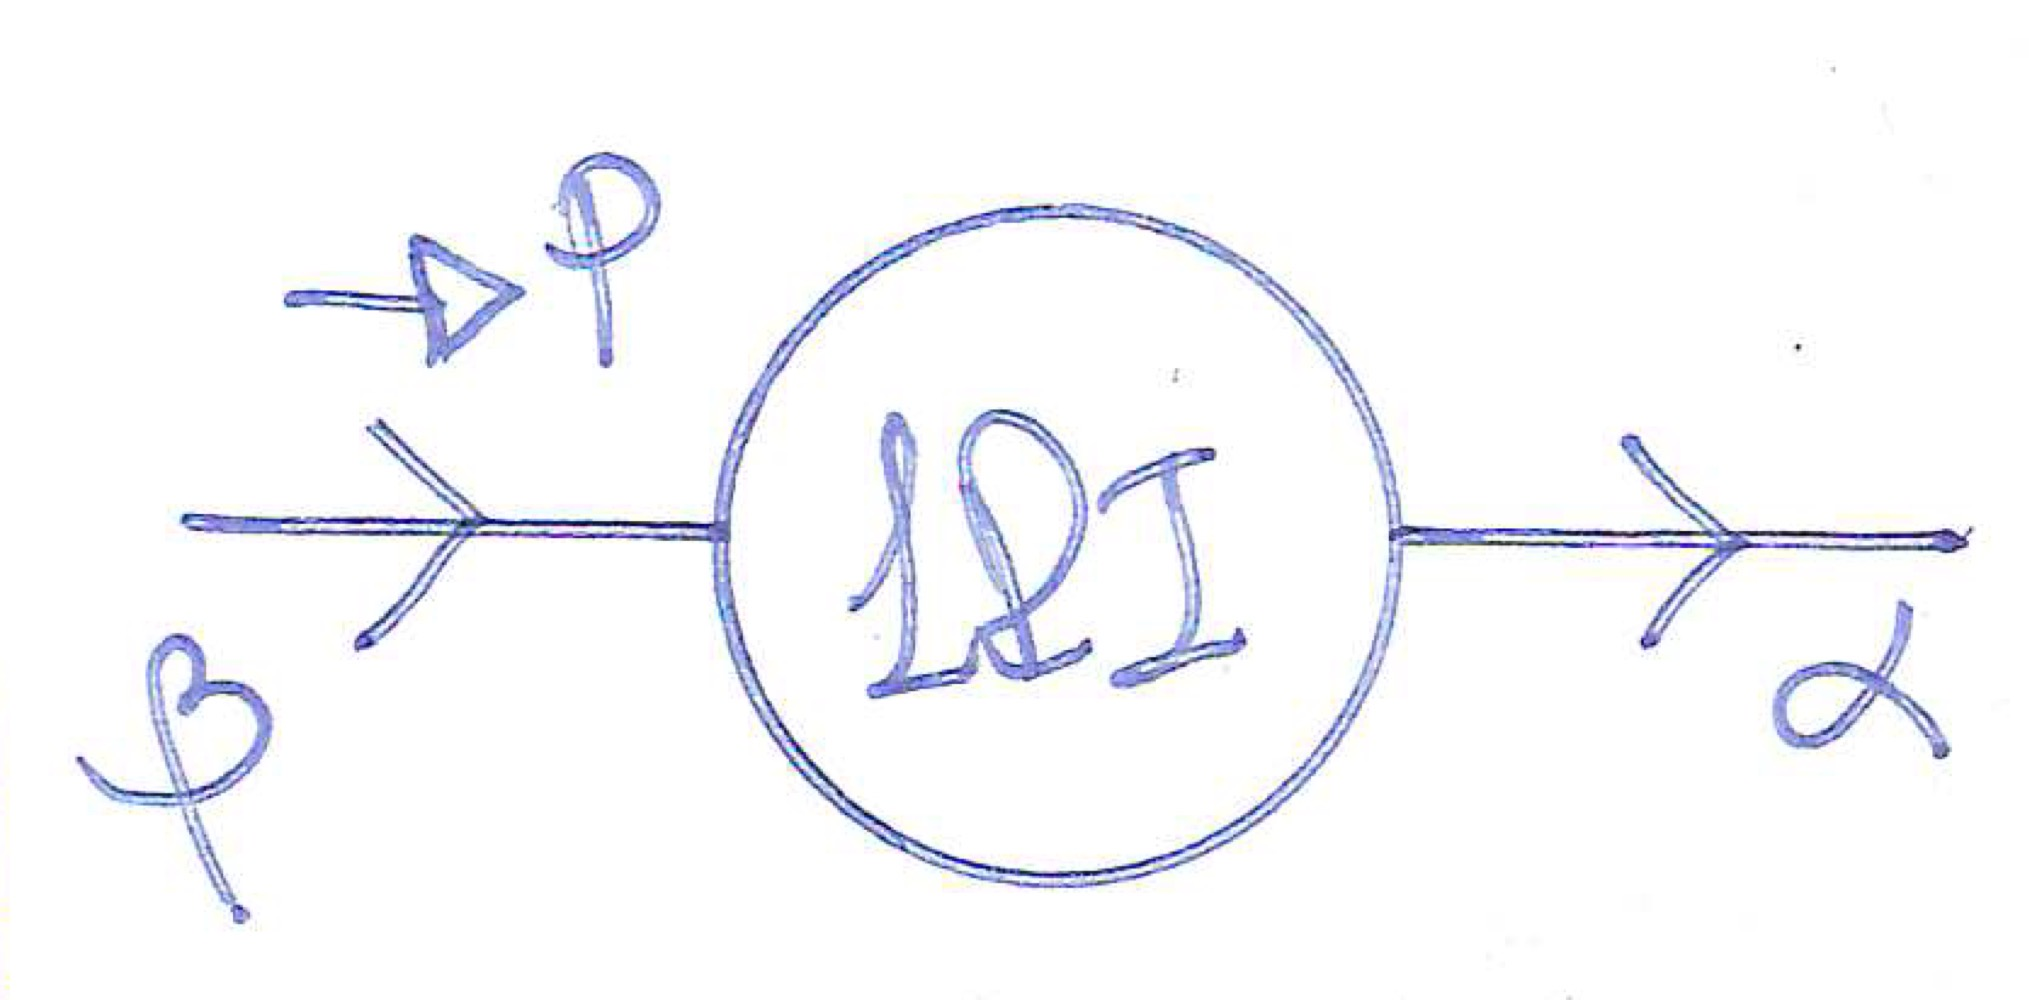
\includegraphics[]{images_ch2/electron_self_energy.JPG}

Un diagramma di questo tipo entra in gioco, ad esempio, come correzione al calcolo dell'ampiezza dello scattering Compton, in cui funge in sostanza da propagatore, quindi off-shell.
Consideriamo quindi spinori non necessariamente on-shell, in modo tale da ottenere un risultato il più generale possibile, da specializzare poi per il caso di interesse.

\subsection{Struttura della soluzione}
La struttura che ci aspettiamo per l'auto-energia dell'elettrone è qualcosa del tipo:
\begin{equation}
    \begin{aligned}
        i\bigl[\Sigma(p)\bigr]_{\alpha\beta} &\sim A(p^2)\delta_{\alpha\beta} + B(p^2)p_\mu\bigl[\gamma^\mu\bigr]_{\alpha\beta} \\
        & = A(p^2)\delta_{\alpha\beta} + B(p^2)\bigl[\slashed p\bigr]_{\alpha\beta}
    \end{aligned}
    \label{eq:ESE_structure}
\end{equation}
Con $A(p^2)$ e $B(p^2)$ funzioni scalari. 

Le motivazioni dietro tale struttura sono le seguenti:
\begin{itemize}
    \item Strutture con più matrici $\gamma$ possono essere sempre riscritte nella forma sopra, se le $\gamma$ sono in numero pari ci si riconduce al termine in $ A(p^2)$, se sono in numero dispari al termine in $B(p^2)$, per esempio:
    \begin{align*}
        C(p^2)p_\mu p_\nu\bigl[\gamma^\mu\gamma^\nu\bigr]_{\alpha\beta} &=  C(p^2)\bigl[\slashed p \slashed p\bigr]_{\alpha\beta}\\
        &= C(p^2)p^2\delta_{\alpha\beta} \\
        & \sim A(p^2)\delta_{\alpha\beta}
    \end{align*}
    \item Il 4-impulso $p^\mu$ entra in gioco solo nella sua forma scalare $p^2$ o in combinazione con le matrici $\gamma$, in quanto $\Sigma$ non ha indici di Lorentz [di conseguenza adotteremo la notazione $\boxed{\Sigma(\slashed p)}$ invece di $\Sigma( p)$].
    \item Non ci aspettiamo combinazioni con la matrice $\gamma_5$, del tipo $a(p^2)\bigl[\gamma_5\bigr]_{\alpha\beta}$ o $b(p^2)\bigl[\gamma_5\gamma^\mu\bigr]_{\alpha\beta}$, per ragioni di parità. 
\end{itemize}

\subsection{Calcolo esplicito ad 1 loop}
Abbiamo un solo diagramma da calcolare, lo chiamiamo $\boxed{i\Sigma_\text{1-loop}(\slashed p)}$
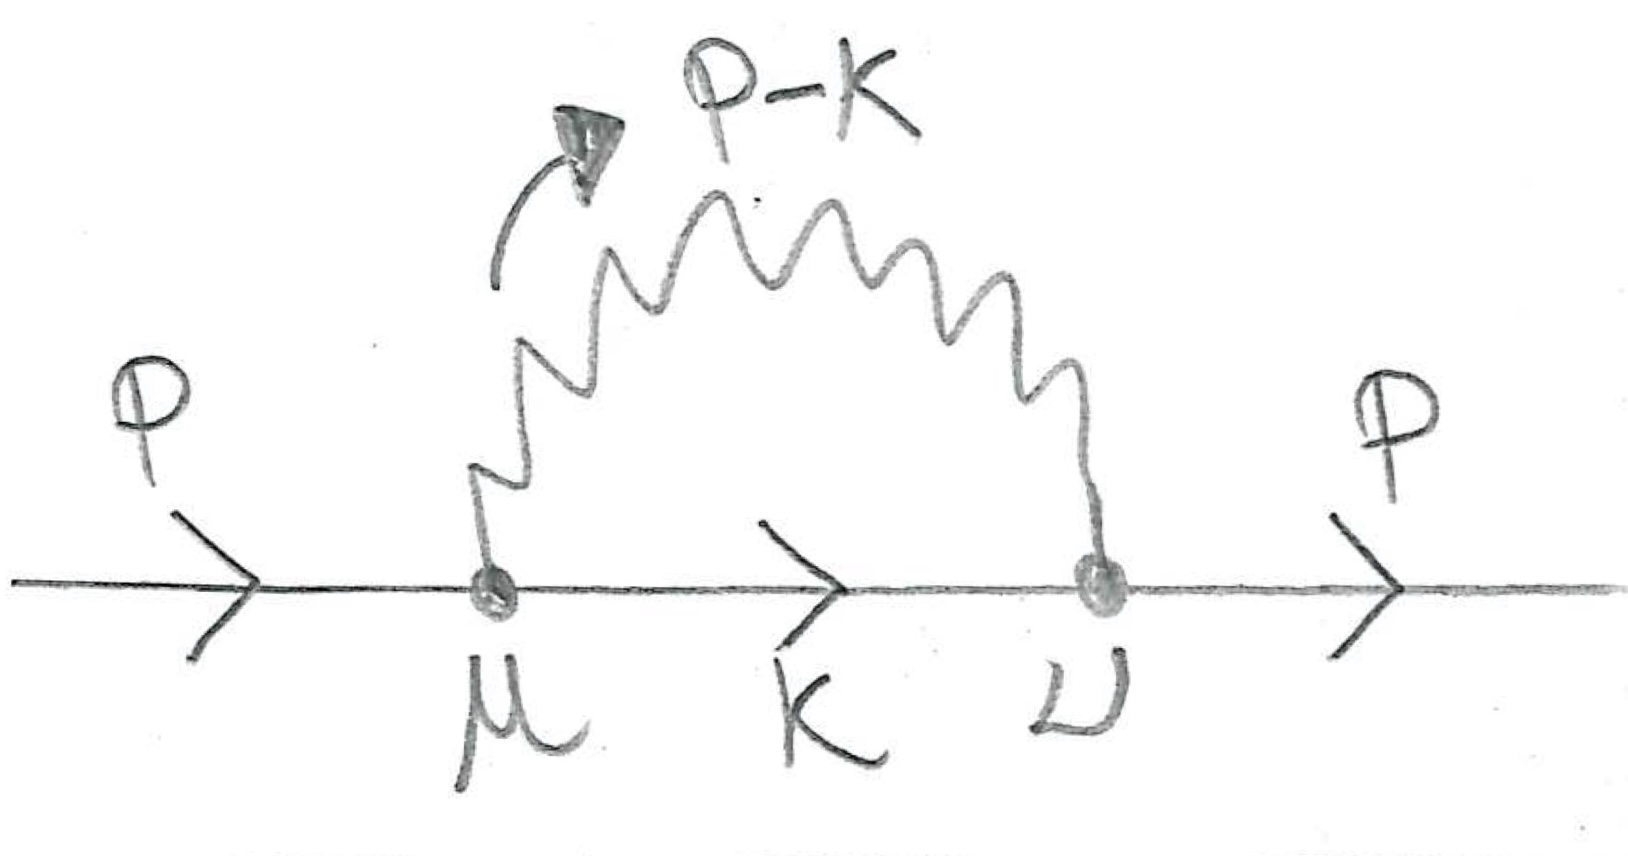
\includegraphics[]{images_ch2/ESE_1loop.jpg}

L'ampiezza che ne risulta, partendo dal vertice $\nu$ è:
\[
i\Sigma_\text{1-loop}(\slashed p) = (ie)^2\int\frac{d^4k}{(2\pi)^4}\bigg[\gamma^\nu\frac{ i(\slashed k + m)}{k^2-m^2+i\varepsilon} \gamma^\mu \frac{(-ig^{\mu\nu})}{(p-k)^2+i\varepsilon}\bigg]
\]

Questi integrali si fanno tutti allo stesso modo. Abbiamo visto i singoli passaggi più nel dettaglio nel caso dell'auto-energia del fotone, nella sezione precedente, quindi cerchiamo di ricavare da questo secondo calcolo una visione più schematica\footnote{a mio parere più utile sul lungo termine, considerato il fatto che difficilmente ci si trova a svolgere a mano questi integrali.}.

\begin{itemize}
    \item[\textcolor{Red}{$\blacktriangleright$}] \textbf{Semplifichiamo l'espressione} 
        \[
        i\Sigma_\text{1-loop}(\slashed p) = (ie)^2\int\frac{d^4k}{(2\pi)^4}\frac{\gamma^\mu (\slashed k + m)\gamma_\mu}{(k^2-m^2+i\varepsilon)[(p-k)^2+i\varepsilon]} \overset{\star}{=}
        \]
    \item[\textcolor{Red}{$\blacktriangleright$}] \textbf{Introduciamo il parametro di Feynman}
        \[
        \overset{\star}{=} (ie)^2\int\frac{d^4k}{(2\pi)^4}\int_0^1 dx \frac{\gamma^\mu (\slashed k + m)\gamma_\mu}{[(1-x)(k^2-m^2+i\varepsilon)+x(p^2 + k^2 -2p\cdot k + i\varepsilon)]^2} \overset{\star}{=}
        \]
    \item[\textcolor{Red}{$\blacktriangleright$}] \textbf{Elaboriamo il denominatore senza il quadrato}
        \begin{align*}
            \sqrt{den} &= k^2(1-x+x) - (1-x)m^2 + xp^2 - 2x\cdot k +i\varepsilon(1-x+x) \\
                       &\overset{\pm x^2p^2}{=} (k-xp)^2 +x(1-x)p^2 - (1-x)m^2 +i\varepsilon
        \end{align*}
    \item[\textcolor{Red}{$\blacktriangleright$}] \textbf{Applichiamo la DIMREG e passiamo in $\mathbf{\mathsf d}$-dimensioni}\\
        In questo modo possiamo invertire l'ordine di integrazione, in quanto considerando $\boxed{\mathsf d < 4}$ l'integrale su $k$ converge.
        Sostituendo anche il denominatore del passaggio precedente otteniamo:
        \begin{align*}
        &\overset{\star}{=} (ie)^2\int_0^1 dx \int\frac{d^\mathsf d k}{(2\pi)^\mathsf d} \frac{\gamma^\mu(\slashed k + m)\gamma_\mu}{[( \underbrace{k-xp}_{\textcolor{Red}{\equiv l}} )^2 \underbrace{+x(1-x)p^2 - (1-x)m^2}_{\textcolor{Blue}{\equiv-\Delta}} +i\varepsilon]^2} \\
        & = (ie)^2\int_0^1 dx \int\frac{d^\mathsf d l}{(2\pi)^\mathsf d} \frac{\gamma^\mu(\slashed l + x\slashed p + m)\gamma_\mu}{[l^2 - \Delta + i\varepsilon]^2} \overset{\star}{=}
        \end{align*}

    \item[\textcolor{Red}{$\blacktriangleright$}] \textbf{Elaboriamo la funzione integranda}\\
        Per farlo sfruttiamo l'algebra di Clifford in ${\mathsf d}$-dimensioni e un paio di identità:
        \[ \{\gamma^\mu, \gamma^\nu \} = 2g^{\mu\nu} ~,~ g^{\mu\nu}g_{\mu\nu}= \mathsf d ~,~ \gamma^\mu\gamma^\nu = \mathsf d\]
        In particolare è facile ricavare:
        \[ \gamma^\mu\gamma^\nu\gamma_\mu = (2-\mathsf d)\gamma^\nu \]
        che ci consente di riscrivere il numeratore dell'integrale, ottenendo:
        \[
        \overset{\star}{=} (ie)^2\int_0^1 dx \int\frac{d^\mathsf d l}{(2\pi)^\mathsf d} \frac{(2-\mathsf d)(\slashed l + x\slashed p) + m \mathsf d}{[l^2 - \Delta + i\varepsilon]^2} \overset{\star}{=}
        \]
    \item[\textcolor{Red}{$\blacktriangleright$}] \textbf{Introduciamo la scala di rinormalizzazione e semplifichiamo i termini che sia annullano per ragioni di parità}
        \[
        \overset{\star}{=} (ie)^2 \mu^{4 - \mathsf d}\int_0^1 dx \int\frac{d^\mathsf d l}{(2\pi)^\mathsf d} \frac{(2-\mathsf d)x\slashed p + m \mathsf d}{[l^2 - \Delta + i\varepsilon]^2} \overset{\star}{=}
        \]
    \item[\textcolor{Red}{$\blacktriangleright$}] \textbf{Effettuiamo una rotazione di Wick: $l^0\rightarrow il^0_E$}\\
        ricordando che, usando la metrica euclidea e definendo $\Vec{l_E} \equiv (l^0, \Vec{l})$, possiamo scrivere $l_E^2 = |\Vec{l_E}|^2 = (l^0)^2 + |\Vec{l}|^2$. Otteniamo quindi, trascurando il termine $i\varepsilon$ in quanto lontani dai poli:
        \begin{align*}
        &\overset{\star}{=} (ie)^2 \mu^{4 - \mathsf d} i \int_0^1 dx \int\frac{d^\mathsf d \Vec{l_E}}{(2\pi)^\mathsf d} \frac{(2-\mathsf d)x\slashed p + m \mathsf d}{[l_E^2 + \Delta]^2} \\
        &= (ie)^2 \mu^{4 - \mathsf d} i \int_0^1 dx [(2-\mathsf d)x\slashed p + m \mathsf d] \underbrace{\int\frac{d^\mathsf d \Vec{l_E}}{(2\pi)^\mathsf d} \frac{1}{[l_E^2 + \Delta]^2}}_{\textcolor{Green}{ \frac{1}{(4\pi)^{\nicefrac{\mathsf d}{2}}} \frac{\Gamma(2-\nicefrac{\mathsf d}{2})}{\Delta^{2-\nicefrac{\mathsf d}{2}}} }} \text{\marginnote{\textcolor{Green}{Sfruttando i risultati notevoli degli integrali Euclidei in ${\mathsf d}$-dimensioni}}} \\
        &\textcolor{Green}{=} (ie)^2 \mu^{4 - \mathsf d} i \int_0^1 dx [(2-\mathsf d)x\slashed p + m \mathsf d] \frac{1}{(4\pi)^{\nicefrac{\mathsf d}{2}}} \frac{\Gamma(2-\nicefrac{\mathsf d}{2})}{\Delta^{2-\nicefrac{\mathsf d}{2}}}  \overset{\star}{=}
        \end{align*} 
        
    \item[\textcolor{Red}{$\blacktriangleright$}] \textbf{Consideriamo la dimensione come una variabile continua ($\mathbf{\mathsf d = 4 - 2\epsilon}$)}\\
    il che implica 
    \[
    2-\mathsf d = -2(1-\epsilon) ~,~ \frac{\mathsf d}{2}=2-\epsilon ~,~ 4-\mathsf d = 2\epsilon
    \]
    L'integrale diventa quindi:
    \begin{align*}
    &\overset{\star}{=}  (ie)^2 \textcolor{cyan}{\mu^{2\epsilon}} i \int_0^1 dx [(-2(1-\epsilon))x\slashed p + m (4-2\epsilon)] \frac{\textcolor{cyan}{(4\pi)^\epsilon}}{(4\pi)^2} \frac{\Gamma(\epsilon)}{\textcolor{cyan}{\Delta^{\epsilon}}}  \\ 
    &\textcolor{cyan}{=} \frac{(ie)^2i}{(4\pi)^2} \int_0^1 dx \bigl[ -2(1-\epsilon)x\slashed p + m (4-2\epsilon) \bigr] \underbrace{\textcolor{cyan}{\bigg(\frac{4\pi \mu^{2}}{\Delta}\bigg)^\epsilon} \Gamma(\epsilon)}_{\frac{1}{\epsilon} - \mathbb\gamma + \log{\frac{4\pi \mu^{2}}{\Delta}} +\mathscr{O}(\epsilon)} \overset{\star}{=}    
    \end{align*}
        
    \item[\textcolor{Red}{$\blacktriangleright$}] \textbf{Scriviamo l'espressione finale}\\
    \begin{equation}
        \begin{aligned}
            &\boxed{
            \begin{aligned}
                    \Sigma_\text{1-loop}(\slashed p) \overset{\star}{=} \frac{(ie)^2}{(4\pi)^2} \int_0^1 dx \Bigl\{&\bigl[ -2(1-\epsilon)x\slashed p +m(4-2\epsilon) \bigr] \times \\ &\bigl[ \frac{1}{\epsilon} - \mathbb\gamma + \log{\frac{4\pi \mu^{2}}{\Delta}} +\mathscr{O}(\epsilon) \bigr] \Bigr\}
            \end{aligned}}\\
        &\Delta \equiv (1-x)(m^2 - xp^2)
        \end{aligned}
        \label{eq:ESE_final}
    \end{equation}
\end{itemize}

Dal confronto (\ref{eq:ESE_structure})$\leftrightarrow$(\ref{eq:ESE_final}) notiamo subito la consistenza con la struttura che abbiamo "tirato a indovinare" all'inizio, basta prendere (trascurando i termini di ordine superiore ad $\mathscr{O}(\epsilon)$)
\begin{align*}
    & A(p^2) = \frac{(ie)^2}{(4\pi)^2} \int_0^1 dx\, 2(2-\epsilon)m \bigg[ \frac{1}{\epsilon} - \mathbb\gamma + \log{\frac{4\pi \mu^{2}}{\Delta}}\bigg]\\
    & B(p^2)  = \frac{(ie)^2}{(4\pi)^2} \int_0^1 dx \,(-2)(1-\epsilon)x \bigg[ \frac{1}{\epsilon} - \mathbb\gamma + \log{\frac{4\pi \mu^{2}}{\Delta}} \bigg]
\end{align*}

Volendo possiamo sistemare meglio queste due funzioni, togliendo di mezzo i termini di $\mathscr{O}(\epsilon)$ che appaiono sviluppando le moltiplicazioni. Scriviamo in definitiva quindi (lasciando gli indici matriciali sottintesi):
\begin{equation}
    \begin{aligned}
    &\boxed{\Sigma_\text{1-loop}(\slashed p) = A(p^2) + \slashed p B(p^2)}\\
       & \begin{aligned} 
            & A(p^2) = \frac{(ie)^2}{(4\pi)^2} \int_0^1 dx\, 4m \biggl[ \frac{1}{\epsilon} - \mathbb\gamma + \log{\frac{4\pi \mu^{2}}{\Delta}} - \frac{1}{2}\biggr]\\
            & B(p^2)  = \frac{(ie)^2}{(4\pi)^2} \int_0^1 dx \,(-2x) \biggl[ \frac{1}{\epsilon} - \mathbb\gamma + \log{\frac{4\pi \mu^{2}}{\Delta}} -1\biggr]
        \end{aligned}
    \end{aligned}
    \label{eq:ESE_structure_revised}
\end{equation}

È evidente come entrambi i termini divergano nel limite $\epsilon \rightarrow 0$ $(\mathsf d = 4)$!

\begin{exercise}
    Calcolare la seguente derivata:
    \[
    \frac{\partial\Sigma_\text{1-loop}(\slashed p)}{\partial \slashed p}\bigg|_{\slashed p = m} = ?
    \]

    Il calcolo di questa derivata è piuttosto lungo e tedioso [lo svolgimento completo è riportato nella \textbf{Lezione 7, p.36÷41}], tuttavia risulterà importante conoscerne il risultato, nell'ottica di riutilizzarlo in seguito.

    \textbf{Spoiler:} il risultato è:
    \begin{equation}
        \frac{\partial\Sigma_\text{1-loop}}{\partial \slashed p}\bigg|_{\slashed p = m} = \frac{e^2}{(4\pi)^2}\bigg[\frac{1}{\epsilon} - \mathbb \gamma + 4 + \log{\frac{4\pi\mu^2}{m^2}} + 2\log{\frac{m_\gamma^2}{m^2}} \bigg]
        \label{eq:ESE_derivative}
    \end{equation}
    Una cosa interessante da notare è che all'interno del calcolo appare un termine con divergenza logaritmica nel limite $k \rightarrow 1$. Questo termine è l'integrale:
    \[
     4m^2\int_0^1 dx \frac{x(2-x)}{(1-x)m^2} = 4m^2\int_0^1 dx \frac{x(2-x)}{\Delta}
    \]
    Questa divergenza è di tipo diverso rispetto a quella ultravioletta: è detta divergenza infrarossa (\textbf{IR}) ed emerge dalla parte dell'integrale al loop in cui $k \rightarrow 0$ (per l'UV $k \rightarrow \infty$).

    In una teoria quantistica di campo generica, le divergenze infrarosse (anche note come \textit{singolarità di massa}) sono associate alla presenza di particelle massless nello spettro. In QED, in particolare, la divergenza IR è associata alla non-massività del fotone.

    Notiamo come, nel caso dell'auto-energia dell'elettrone, la divergenza IR appaia nel calcolo della derivata di $\Sigma(\slashed p)$, quindi se ne deduce che, in prima approssimazione, $\Sigma(\slashed p)$ non diverge in IR. La divergenza emerge solo considerando la correzione al prim'ordine.

    La procedura di regolarizzazione della divergenza infrarossa consiste nell'introdurre a mano un termine al denominatore del propagatore del fotone nell'ampiezza iniziale: "$-m_\gamma^2$". Il nome non è scelto a caso: introdotto in questo modo, il termine $m_\gamma$ assume a tutti gli effetti il ruolo di massa del fotone (una massa fittizia chiaramente, il fotone non ha massa.).

    In formule, l'ampiezza diventa:
    \[
    i\Sigma_\text{1-loop}(\slashed p) = (ie)^2\int\frac{d^4k}{(2\pi)^4}\frac{\gamma^\nu i(\slashed k + m)\gamma^\mu(-ig^{\mu\nu})}{(k^2-m^2+i\varepsilon)\bigl[(p-k)^2-m_\gamma^2+i\varepsilon\bigr]}
    \]
    E ripetendo le solite tecniche di calcolo degli integrali al loop, quello che cambia è la definizione di $\Delta$ al momento dell'introduzione del parametro di Feynman. Si trova:
    \[\Delta = (1-x)(m^2-xp^2) \textcolor{Blue}{+xm_\gamma^2}\]
    Il gioco è fatto! Ora la massa del fotone agisce come cutoff per l'integrale e quest'ultimo può essere calcolato senza alcuna difficoltà.

    Inoltre la scomparsa della divergenza contestualmente all'inserimento di una massa $m_\gamma \neq 0$ è una conferma del fatto che la divergenza infrarossa sia originata dalla non-massività del fotone.
    \label{ex:dSigma_dpslashed}
\end{exercise}

\section{La funzione vertice}
Consideriamo il vertice di QED generico, in cui espandiamo il punto di interazione in modo da tenere conto di possibili correzioni al loop. Chiamiamo questa ampiezza \textbf{Funzione Vertice}, la indichiamo con "$ie\bigl[ \Gamma^\mu(q_1,q_2)\bigr]_{\alpha\beta}$" e la rappresentiamo come segue:

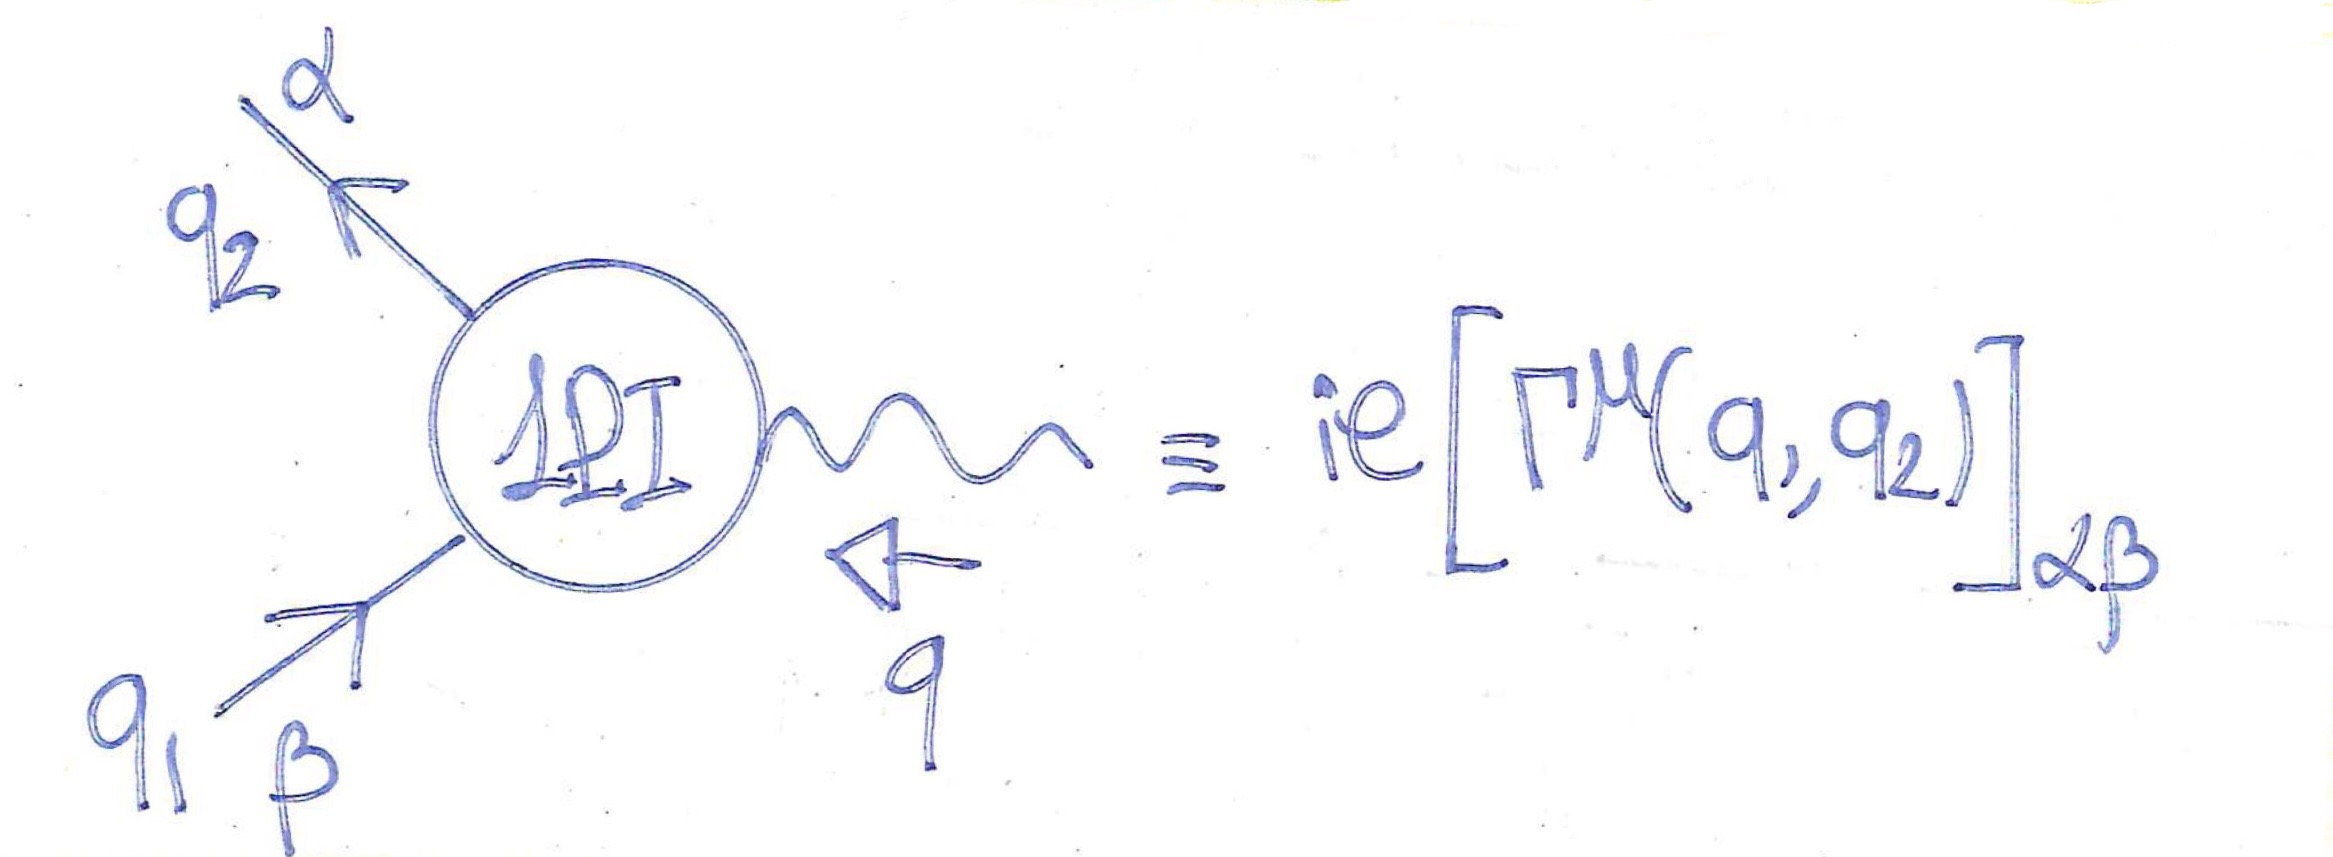
\includegraphics[]{images_ch2/vertex_function.jpg}

Possiamo subito osservare come il grado di divergenza sia $D=0$ e come la conservazione globale dell'impulso forzi la condizione:
\[q_1 + q = q_2 \Rightarrow q = q_2 - q_1 \]

\begin{nota}
    Nel momento in cui volessimo includere spinori esterni e considerando il fotone come on-shell scriveremmo:
    \[
    i\mathscr{M} =\bar u_\alpha(q_2) ie\bigl[ \Gamma^\mu(q_1,q_2)\bigr]_{\alpha\beta} u_\beta(q_1) \varepsilon_\mu(q)
    \]
    Quindi $\Gamma_\mu$ è una matrice $4\times4$ con un indice da 4-vettore ($\mu$).
    
    \marginnote{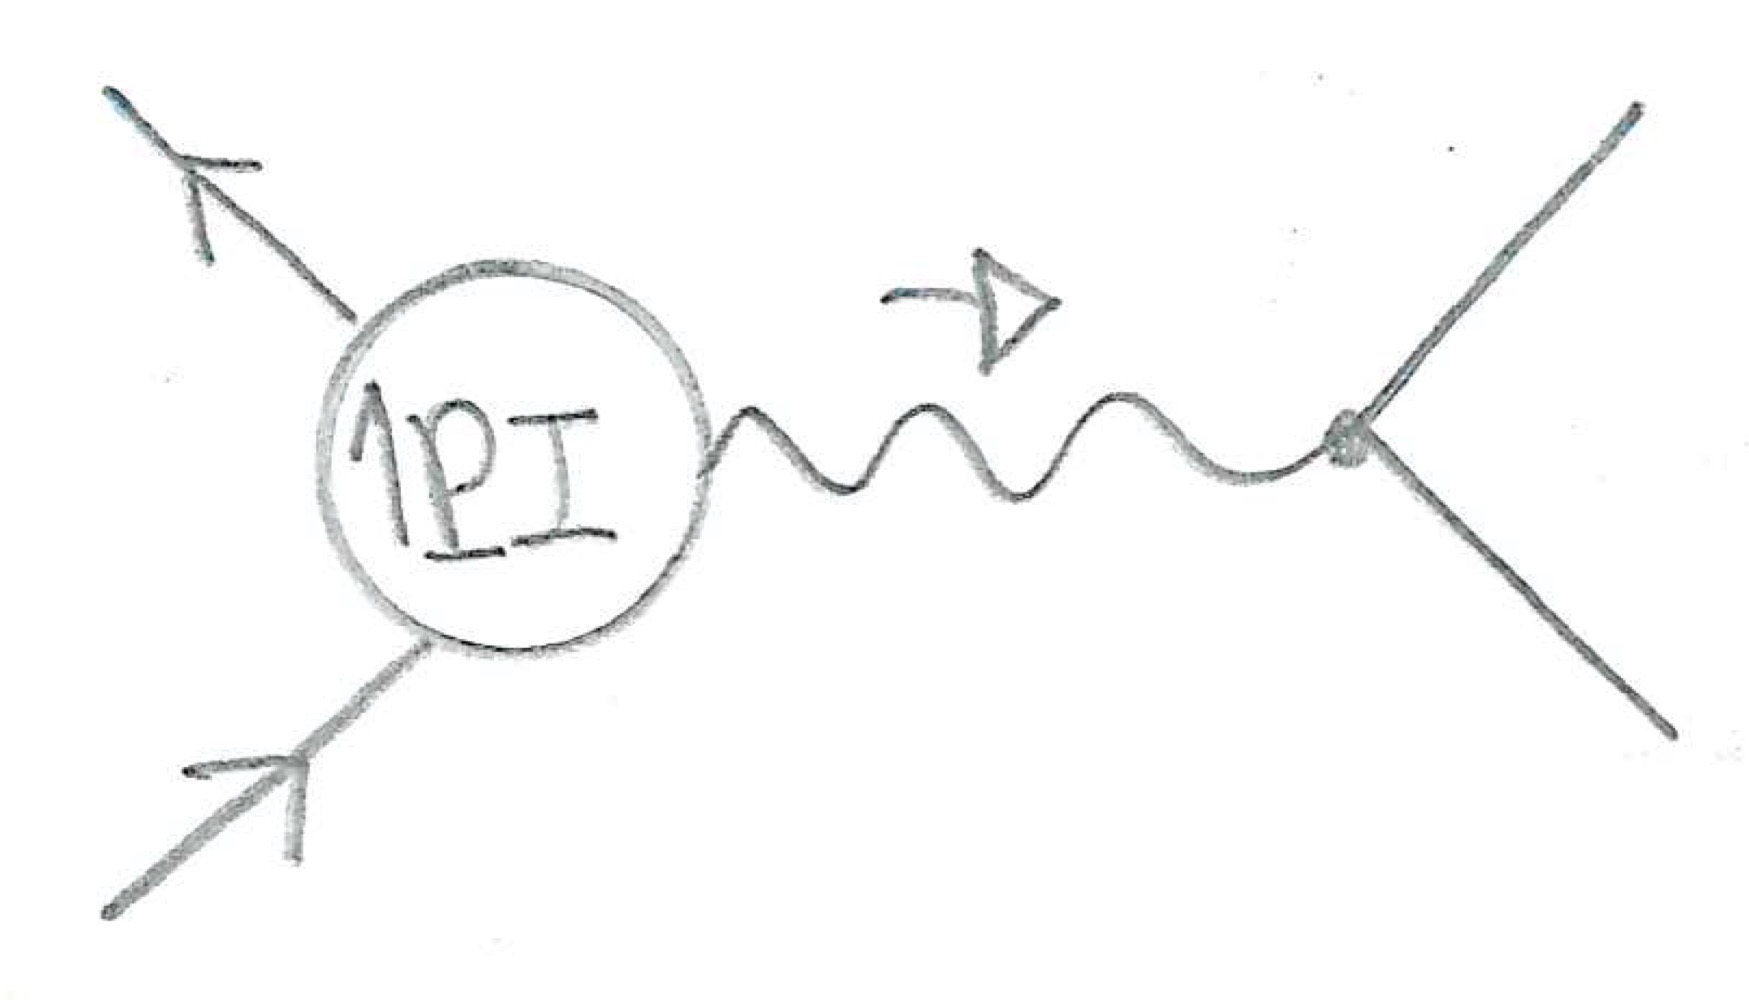
\includegraphics[]{images_ch2/vertex_correction.jpg}}
    
    Come al solito, non facciamo assunzioni sulla natura del fotone esterno, ci sono infatti casi in cui la funzione vertice appare come correzione in diagrammi che coinvolgono un fotone come propagatore dell'interazione (ne è un esempio il diagramma al lato), quindi cercheremo di tenerci il più generali possibili, concentrandoci solo su $i\Gamma^\mu$ e trascurando vettori di polarizzazione o spinori esterni.
\end{nota}
\subsection{I Fattori di Forma}
Partiamo da alcune \textcolor{Orange}{\textbf{considerazioni generiche}} sulla struttura di $i\Gamma^\mu(q_1,q_2)$:
\begin{itemize}
    \item[\textcolor{Orange}{$\blacksquare$}] \textbf{Covarianza di Lorentz}\\
        Considerato il fatto che $\Gamma^\mu$ ha un indice di Lorentz, la sua struttura dovrà necessariamente coinvolgere $q_1^\mu$. $q_2^\mu$ e $\gamma^\mu$; inoltre, ci aspettiamo che la natura matriciale emerga dai coefficienti di questi tre componenti principali:
        \[
        \bigl[\Gamma^\mu(q_1,q_2)\bigr]_{\alpha\beta} = A_{\alpha\beta}q_1^\mu + B_{\alpha\beta}q_2^\mu + \bigl(C\gamma^\mu\bigr)_{\alpha\beta}
        \]

        La struttura più generica che possiamo quindi scrivere è la seguente, dove omettiamo gli indici $\alpha$ e $\beta$ per semplicità:
        \begin{equation}
            \begin{aligned}
            \Gamma^\mu(q_1,q_2) = & (A_1 + A_2\slashed q_1 + A_3\slashed q_2 + A_4\slashed q_1 \slashed q_2)q_1^\mu\\
                                  & (B_1 + B_2\slashed q_1 + B_3\slashed q_2 + B_4\slashed q_1 \slashed q_2)q_2^\mu\\
                                  & (C_1\gamma^\mu + C_2\gamma^\mu\slashed q_1 + C_3\slashed q_2\gamma^\mu + C_4\slashed q_2 \gamma^\mu \slashed q_1)
            \end{aligned}
            \label{eq:vertex_amplit_genericstructure}
        \end{equation}
        con $A_i$, $B_i$, $C_i$ funzioni scalari di $q_1^2$, $q_2^2$ e $q_1\cdot q_2$. Ogni alta combinazione può essere riscritta nella forma sopra per mezzo di identità quali $\slashed q_1\slashed q_1 = q_1^2$ o $\slashed q_1\slashed q_2 = \slashed q_2\slashed q_1 + 2q_1\cdot q_2$.
        
    \item[\textcolor{Orange}{$\blacksquare$}] \textbf{Fermioni on-shell}\\
        È fuori da ogni dubbio che la forma generica (\ref{eq:vertex_amplit_genericstructure}) per $\Gamma^\mu(q_1,q_2)$ sia piuttosto complicata. Per semplificare la trattazione, assumiamo che $\Gamma^\mu(q_1,q_2)$ appaia sempre in un sandwich tra due spinori on-shell, i.e.: 
        \begin{equation}
            \bar u(q_2) ie\Gamma^\mu(q_1,q_2) u(q_1)
            \label{eq:vertex_sandwich}
        \end{equation}

        \begin{nota}
            Potrebbe sembrare una limitazione, soprattutto rispetto a quanto detto poc'anzi in merito alla volontà di mantenere la discussione il più generica possibile, ed in effetti da un lato lo è: se dovessimo trovarci a trattare le correzioni allo scattering Compton\marginnote{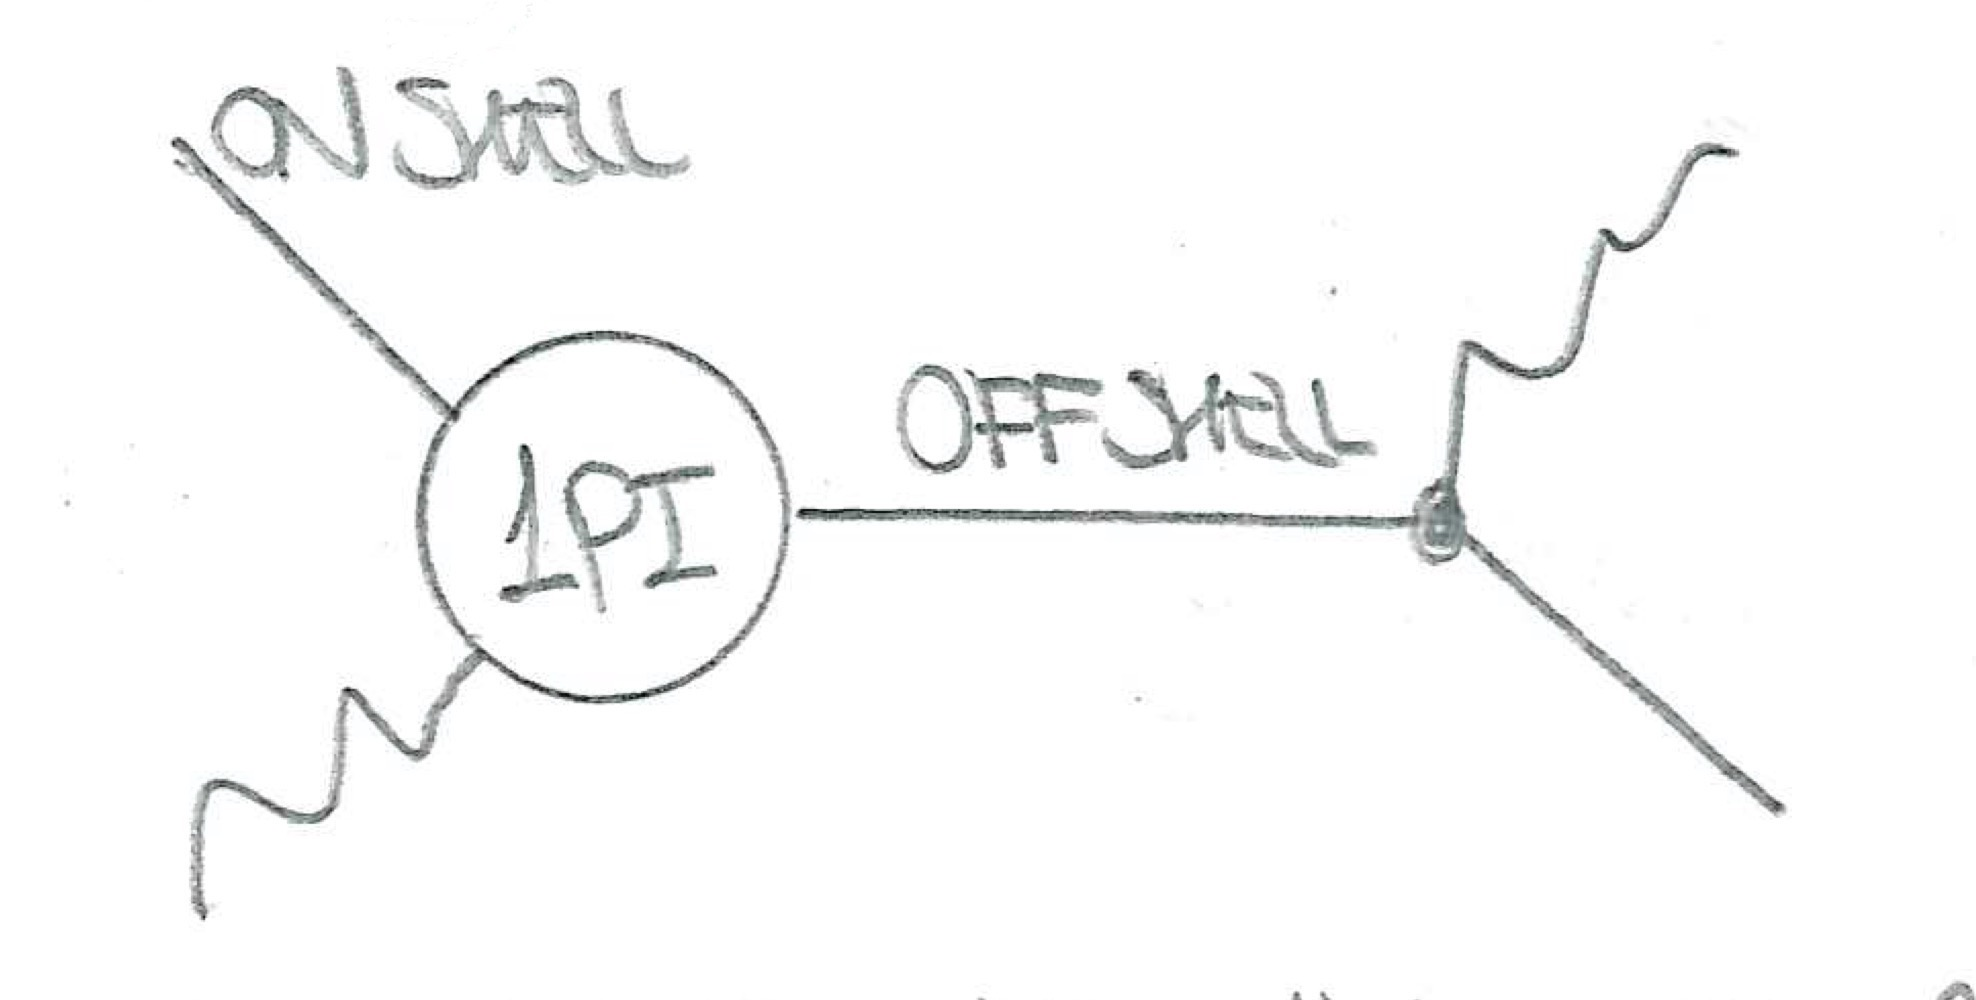
\includegraphics[]{images_ch2/compton_vertex_correction.jpg}}, ci troveremmo con solo uno dei due spinori on-shell (quello esterno), mentre il secondo è chiuso in un propagatore off-shell. Questo ci impedirebbe di inserire tale oggetto nella nostra trattazione.\\

            Tuttavia, finché la procedura di rinormalizzazione resta nell'equazione globale (i.e. finché la parte UV-divergenza del diagramma viene cancellata) non c'è alcuna perdita di generalità nel assumere che gli indici $\alpha$ e $\beta$ siano connessi a spinori on-shell.\footnote{In seguito verrà fatta maggiore chiarezza al riguardo. Per ora basti sapere che si tratta di una semplificazione, anche se non del tutto evidente.}
        \end{nota}
        Due principali semplificazioni emergono da questa assunzione:
        \begin{enumerate}
            \item Essendo i fermioni esterni on-shell, vale la legge secondo cui $q_1^2=q_2^2=m^2$. Segue       immediatamente, tenendo conto della conservazione del 4-impulso:
                \[
                q^2 = 2m^2 - 2q_1\cdot q_2
                \]
                Possiamo quindi dire che $A_i$, $B_i$ e $C_i$ sono funzioni solo di $q^2$ ed $m^2$
            \item Dall'equazione di Dirac possiamo ricavare:
                \[
                \begin{aligned}
                    (\slashed q_1 - m)u(q_1) &= 0\\
                    \bar u(q_2)(\slashed q_2 - m) &= 0 
                \end{aligned}
                \,\Rightarrow\,
                \boxed{
                \begin{aligned}
                    \slashed q_1 u(q_1) &= m u(q_1)\\
                    \bar u(q_2)\slashed q_2 &=  \bar u(q_2)m
                \end{aligned}
                }\]
                A questo punto, se esplicitiamo la forma generale di $\Gamma^\mu$ nel sandwich, ci accorgiamo del fatto che, per mezzo dell'equazione di Dirac, tutti i vettori slashed possono essere sostituiti con $m$. Raccogliendo i termini in parentesi in singole funzioni più generiche otteniamo:
                \begin{equation}
                    \Gamma^\mu(q_1,q_2) = A(q^2)q_1^\mu + B(q^2)q_2^\mu +C(q^2)\gamma^\mu
                    \label{eq:vertex_amplit_revisedstructure}
                \end{equation}
        \end{enumerate}
        
    \item[\textcolor{Orange}{$\blacksquare$}] \textbf{Identità di Ward}\\
        Consideriamo un ampiezza di scattering generica
        \[ 
        i\mathscr{M}=\bigl[\bar u(q_2) ie\Gamma^\mu(q_1,q_2) u(q_1)\bigr]\varepsilon_\mu(q) 
        \]
        ed assumiamo il fotone come on-shell\footnote{In realtà l'identità di Ward vale anche nel caso in cui i fotoni siano off-shell, come nel caso della correzione per lo scattering Compton.} con 4-impulso $q_\mu$.

        Questo ci permette di effettuare la sostituzione $\varepsilon_\mu(q)\rightarrow \varepsilon_\mu(q) + C_\lambda q_\mu$\footnote{$C_\lambda$ è un fattore che non ci interessa ed il perché di questa sostituzione può essere compreso studiando la derivazione dell'equazione (\ref{eq:generalized_polvec}), ma la sostanza è che ciò è conseguenza dell'invarianza di gauge.}, ottenendo due termini, il primo identico ad $i\mathscr{M}$ e che cancella il LHS, mentre il secondo non è altro se non l'identità di Ward:
        \begin{equation} 
        \bigl[\bar u(q_2) ie\Gamma^\mu(q_1,q_2) u(q_1)\bigr]q_\mu \overset{!}{=} 0 
        \label{eq:ward_id_vertex}
        \end{equation}
        Esplicitando la struttura di $\Gamma^\mu$ secondo la (\ref{eq:vertex_amplit_revisedstructure}) e sfruttando la condizione di fermioni on-shell, l'equazione di Dirac e la conservazione dell'impulso, si arriva facilmente al seguente risultato:
        \[\bigl[\bar u(q_2) (q_1\cdot q_2 - m^2) (A-B) u(q_1)\bigr]q_\mu \overset{!}{=} 0 \]
        da cui segue che 
        \[\boxed{A(q^2)=B(q^2)}\]

        Di conseguenza la struttura della funzione vertice diventa:
        \begin{equation}
            \marginnote{\textbf{Nota:} questa espressione è valida per fermioni on-shell e fotoni off-shell.}
            \boxed{\Gamma^\mu(q_1,q_2) = A(q^2)(q_1 + q_2)^\mu +C(q^2)\gamma^\mu} 
            \label{eq:vertex_amplit_revisedstructure2}
        \end{equation}
        Dove $A(q^2)$ e $C(q^2)$ sono detti \textbf{Fattori di Forma}.
    
    \item[\textcolor{Orange}{$\blacksquare$}] \textbf{Identità di Gordon}\\
        Enunciamo innanzitutto suddetta identità:
        \begin{equation}
            \begin{aligned}
                2m\, \bar u(q_2)\gamma^\mu u(q_1) = &\bigl(q_2 + q_1\bigr)^\mu \, \bar u(q_2) u(q_1) \\
                                                 & + i \bigl(q_2 - q_1\bigr)_\nu \, \bar u(q_2)\sigma^{\mu\nu} u(q_1)
            \end{aligned}
            \label{eq:gordon_identity}
        \end{equation}
        con $\sigma^{\mu\nu} \equiv \frac{i}{2}\bigl[\gamma^\mu,\gamma^\nu\bigr]$
        \begin{exercise}
            Dimostrare l'identità di Gordon (\ref{eq:gordon_identity}).
            
            [\textbf{svolto Lezione 8 p.48}]
        \end{exercise}

        A questo punto l'idea è quella di sfruttare l'identità di Gordon per riscrivere in maniera diversa i termini di $\Gamma^\mu(q_1,q_2)$.

        Partiamo dal sandwich (\ref{eq:vertex_sandwich}) e inseriamo l'espressione (\ref{eq:vertex_amplit_revisedstructure2}), separiamo i termini in $A(q^2)$ e $C(q^2)$ e, riconoscendo nel coefficiente di $A(q^2)$ il primo termine dell'identità di Gordon, invertiamo quest'ultima ed effettuiamo la sostituzione.
        Un opportuno ri-arrangiamento dei termini ci porta alla forma:
        \[
        \bar u(q_2) \Gamma^\mu(q_1,q_2) u(q_1) = \bar u(q_2) \bigl[ F_1(q^2)\gamma^\mu +\frac{i\sigma^{\mu\nu}q_\nu}{2m} F_2(q^2) \bigr] u(q_1)
        \]

        da cui segue
        
        \begin{equation}
            \boxed{
            \Gamma^\mu(q_1,q_2) = \underbrace{F_1(q^2)}_{\substack{\text{Fattore}\\\text{di Forma}\\ \text{Elettrico}}}\gamma^\mu +\frac{i\sigma^{\mu\nu}q_\nu}{2m} \underbrace{F_2(q^2)}_{\substack{\text{Fattore}\\\text{di Forma}\\ \text{Magnetico}}}
            }
            \label{eq:vertex_formfactors}
        \end{equation}
        con
        \begin{equation}
            \boxed{
            \begin{aligned}
                &F_1(q^2) = 2mA(q^2) + C(q^2) \\
                &F_2(q^2) = -2mA(q^2)
            \end{aligned}
            }
            \label{eq:formfactors}
        \end{equation}
    
    \item[\textcolor{Orange}{$\blacksquare$}] \textbf{Considerazioni riguardo la divergenza UV}\\
        Ricordiamo che il grado di divergenza della funzione vertice è $D=0$. Se espandiamo rispetto all'impulso esterno $q$ possiamo scrivere:
        \[
        \Gamma^\mu(q_1,q_2) \approx \underbrace{F_1(q^2=0)\gamma^\mu}_{D=0} + \underbrace{\Bigl[ \frac{\partial F_1}{\partial q^\nu}\bigg|_{q=0}\gamma^\mu + \frac{i\sigma^{\mu}_{~\nu}}{2m} F_2(q^2=0)\Bigr]q^\nu + \cdot\cdot\cdot}_{D<0} 
        \]
        In sostanza ci aspettiamo che la divergenza arrivi solo dalla parte che concerne il fattore di forma elettrico!
\end{itemize}
\subsection{Calcolo esplicito ad 1 loop}
\begin{itemize}
    \item [\textcolor{Black}{$\blacksquare$}]\textbf{Considerazioni preliminari: il Tree-level}\\
        Tenendo conto al massimo delle correzioni ad un loop, possiamo decomporre la funzione vertice in una somma di due diagrammi:
        
        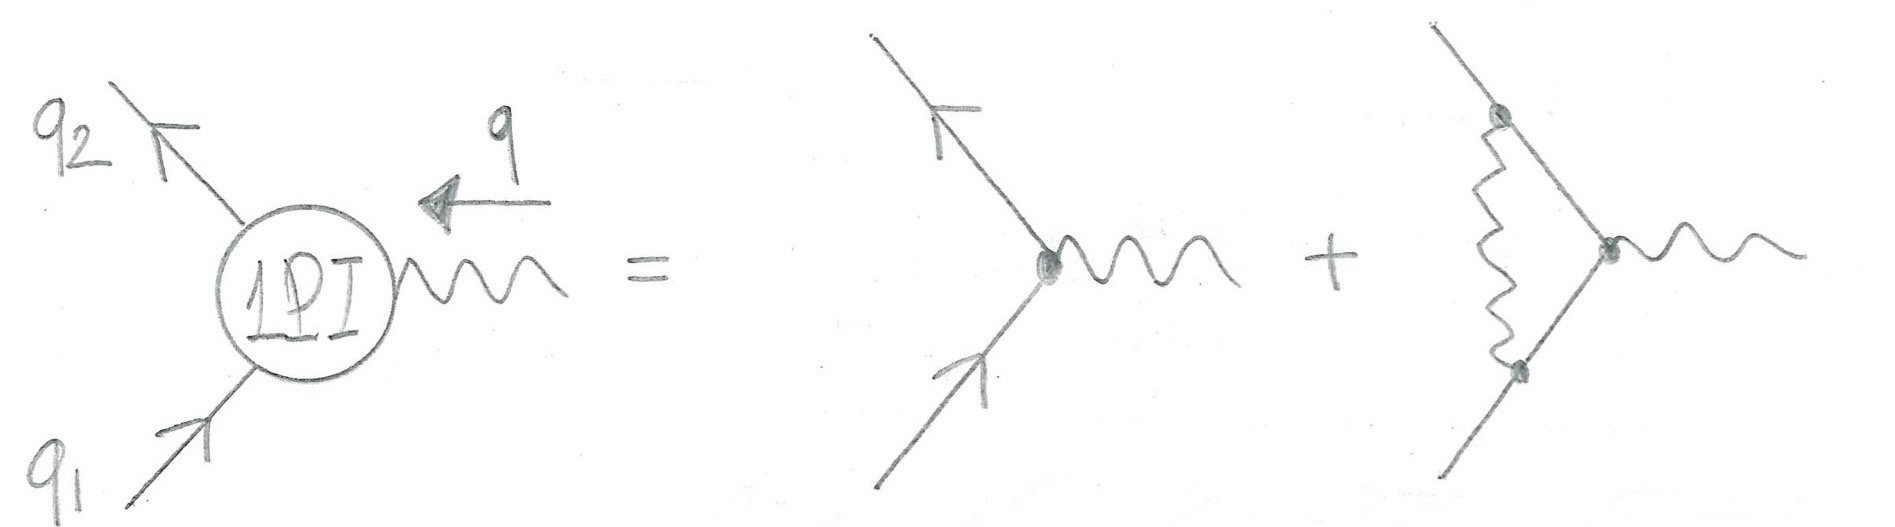
\includegraphics[]{images_ch2/vertex_decomposition.jpg}

        Se confrontiamo la struttura (\ref{eq:vertex_formfactors})\footnote{chiaramente, moltiplicata per $ie$}, che abbiamo appena derivato, con quella del termine al tree-level ($ie\gamma^\mu$) troviamo:
        \begin{equation}
            F_{1, \text{TREE}}(q^2) = 1; ~~~ F_{2, \text{TREE}}(q^2) = 0 ~~~\forall\,q^2
            \label{eq:formfactors_treelevel}
        \end{equation}
    \item [\textcolor{Black}{$\blacksquare$}]\textbf{Il vertice a un loop}\\
    Concentriamoci ora sul termine a un loop, il diagramma da calcolare è il seguente:
    
    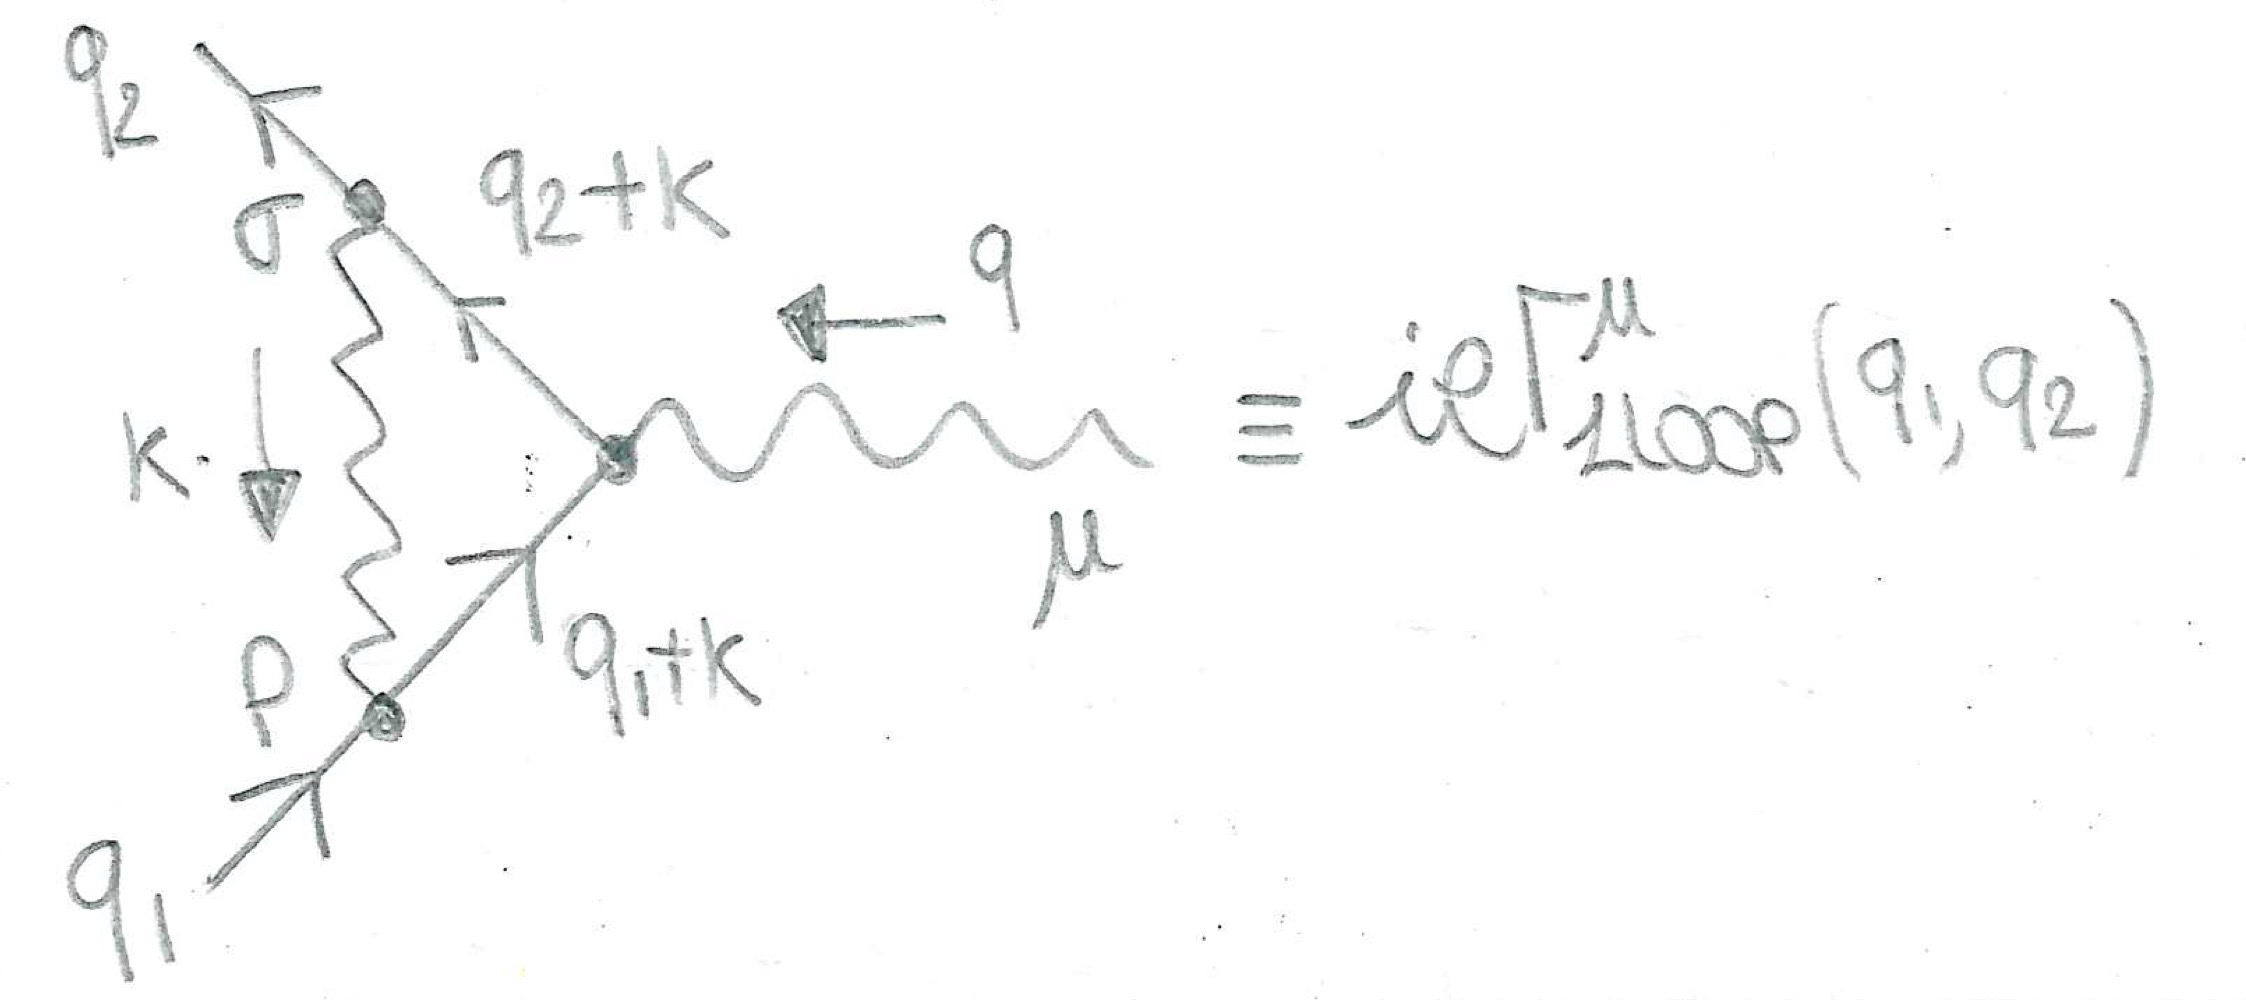
\includegraphics[]{images_ch2/vertex_oneloop.JPG}

    e l'ampiezza che ne deriva può essere scritta come segue, partendo dal propagatore fotonico verticale a sinistra:
    \begin{equation}
        \begin{aligned}
           ie\Gamma^\mu_\text{1-loop}(q_1,q_2) = (ie)^3\int \frac{d^4k}{(2\pi)^4} \Bigg\{& \frac{(-ig^{\rho\sigma})}{k^2+i\varepsilon} \gamma^\sigma\cdot  \\
           \cdot&\frac{i(\slashed q_2 + \slashed k + m)}{\bigl[( q_2 +  k)^2 - m^2 + i\varepsilon\bigr]}\gamma^\mu\cdot \\ 
           \cdot&\frac{i(\slashed q_1 + \slashed k + m)}{\bigl[( q_1 + k)^2 - m^2 + i\varepsilon\bigr]}\gamma^\rho \Bigg\}
        \end{aligned}
        \label{eq:vertex_amplit_oneloop}
    \end{equation}

    Anche in questo caso, come nei due precedenti, i passaggi da svolgere sono sempre gli stessi, con alcune complicazioni dovute alla presenza di 3 vertici di interazione, ma lo spirito è il medesimo.

    Lasciamo quindi al lettore volenteroso il divertimento dello svolgimento esplicito e delineiamo i \textcolor{Red}{passaggi chiave}, senza formule:
    \begin{itemize}
        \item[\textcolor{Red}{$\blacktriangleright$}] Sistemiamo la funzione integranda e introduciamo i parametri di Feynamn (che questa volta sono 3);
        \item[\textcolor{Red}{$\blacktriangleright$}] Applichiamo la regolarizzazione dimensionale e rielaboriamo il numeratore sfruttando alcune proprietà delle matrici gamma in $\mathsf d$-dimensioni;
        \item[\textcolor{Red}{$\blacktriangleright$}] Cambiamo variabile di integrazione;
        \item[\textcolor{Red}{$\blacktriangleright$}] Utilizziamo la condizione on-shell (questo passaggio è nuovo, negli altri due casi non abbiamo sfruttato tale assunzione);
        \item[\textcolor{Red}{$\blacktriangleright$}] Applichiamo la riduzione tensoriale al primo termine
        \item[\textcolor{Red}{$\blacktriangleright$}] Arriviamo al risultato finale:
            \marginnote{Osserviamo come questa risultato sia perfettamente compatibile con quello tirato ad indovinare passando per l'identità di Ward (\ref{eq:vertex_amplit_revisedstructure2}).}
            \begin{equation}
               \boxed{ 
               \begin{aligned}
                   ie\Gamma^\mu_\text{1-loop}(q_1,q_2) = (ie)^2i&\int dxdydz \,\delta(x+y+z-1) \\ 
                   &\times\int \frac{d^\mathsf d l}{(2\pi)^\mathsf d } \frac{2\mathscr{N}^\mu}{(l^2-\Delta+i\varepsilon)^3}
               \end{aligned}}
                \label{eq:vertex_amplit_oneloop_final1}
            \end{equation}
            dove
            \begin{equation}
            \begin{aligned}
                &\begin{aligned}
                       \mathscr{N}^\mu =\Bigg\{ & \frac{(\mathsf d-2)^2}{\mathsf d}l^2\gamma^\mu +m^2\gamma^\mu\bigl[ 4z - (\mathsf d - 2)(1-z)^2 \bigr]\\
                       & - q^2\gamma^\mu\bigl[ 2z + (\mathsf d - 2)xy \bigr] \\
                       & - im\sigma^{\mu\nu}q_\nu(1-z)\bigl[ 2z + (4-\mathsf d)(1-z) \bigr]\Bigg\}
                \end{aligned}\\
                &\Delta = (1-z)^2m^2 - xyq^2
            \end{aligned}
            \end{equation}
    \end{itemize}
    \item [\textcolor{Black}{$\blacksquare$}]\textbf{Risultato del calcolo in funzione dei fattori di forma}\\
        Possiamo riscrivere il risultato precedente in funzione dei Fattori di Forma (elettrico e magnetico) imponendo (\ref{eq:vertex_formfactors}) $\overset{!}{=}$ (\ref{eq:vertex_amplit_oneloop_final1}), il che ci permette di trovare:
        \begin{equation}
            \boxed{
            \begin{aligned}
                &\begin{aligned}
                F_{1,\text{1-loop}}(q^2) = -2ie^2&\int_0^1 dxdydz \,\delta(x+y+z-1) \\ 
                       &\times\int \frac{d^\mathsf d l}{(2\pi)^\mathsf d} \frac{\mathscr{N}_1}{(l^2-\Delta+i\varepsilon)^3}
                \end{aligned}\\
                &\begin{aligned}
                       \mathscr{N}_1 =\Bigg\{ \frac{(\mathsf d-2)^2}{\mathsf d}l^2 &+ m^2\bigl[ 4z - (\mathsf d - 2)(1-z)^2 \bigr]\\
                       & - q^2\bigl[ 2z + (\mathsf d - 2)xy \bigr]\Bigg\}
                \end{aligned}
            \end{aligned}}
            \label{eq:formfactor1_final}
        \end{equation}
        
        \begin{equation}
            \boxed{
            \begin{aligned}
                &\begin{aligned}
                F_{2,\text{1-loop}}(q^2) = +2ie^2&\int_0^1 dxdydz \,\delta(x+y+z-1) \\ 
                       &\times\int \frac{d^\mathsf d l}{(2\pi)^\mathsf d} \frac{\mathscr{N}_2}{(l^2-\Delta+i\varepsilon)^3}
                \end{aligned}\\
                &\begin{aligned}
                       \mathscr{N}_2 = 2m^2(1-z)\bigl[ 2z + (4-\mathsf d)(1-z) \bigr]
                \end{aligned}
            \end{aligned}}
            \label{eq:formfactor2_final}
        \end{equation}
\end{itemize}
Quindi, il risultato che abbiamo ottenuto è perfettamente compatibile con entrambe le strutture che abbiamo tirato ad indovinare in principio! 

Inoltre, notiamo che l'unica parte divergente è $F_{1,\text{1-loop}}$ e che in particolare il termine divergente risulta essere:
\[
 F_{1,\text{1-loop}}\supset -2ie^2\int_0^1 dxdydz \,\delta(x+y+z-1)\int \frac{d^\mathsf d l}{(2\pi)^\mathsf d}\frac{(\mathsf d-2)^2}{\mathsf d(l^2-\Delta+i\varepsilon)^3}l^2
\]

\begin{exercise}
    Calcolare $F_{1,\text{1-loop}}(q^2=0)$.\\
    \textbf{Soluzione (Sketch):} Ancora una volta ci troviamo a voler calcolare un integrale al loop ed il procedimento è grossomodo lo stesso. Inoltre, come già visto nell'esercizio \ref{ex:dSigma_dpslashed}, anche in questo caso appare un termine divergente in infrarosso, per cui risulta necessario introdurre la massa fittizia del fotone per porre un cutoff a tale divergenza. 
    
    Al solito quindi:
    \begin{itemize}
        \item Effettuiamo una rotazione di Wick $l^0 \rightarrow il^0_E$.
        \item Utilizziamo gli integrali Euclidei noti in $\mathsf d$-dimensioni e riportiamo in $\mathsf d=4$ quelli che            vediamo essere convergenti in tal limite. 
        \item A questo punto ci troviamo a dover calcolare due integrali:
        \begin{enumerate}
            \item Regolarizziamo l'integrale IR-divergente (che è quello in $dz$ quando $z\rightarrow 1$) e poi integriamo sui tre parametri di Feynman grazie alla $\delta(x+y+z-1)$.
            \marginnote{la $\delta$ ci permettere di togliere una delle variabili, ma dobbiamo ricordarci dei limiti di integrazione! Infatti \[0\leq y\overset{\delta}{=} 1-x-z\leq 1\] implica
            \[
            \begin{cases}
            1-x-z\leq 1\\
            1-x-z\geq 0
            \end{cases} \Rightarrow
            \begin{cases}
            x+z\geq 0\\
            x\leq 1-z
            \end{cases}
            \]}
            \item Per il calcolo dell'integrale rimasto consideriamo la dimensione come variabile continua $\mathsf d = 4 -2\epsilon$, introduciamo al scala di rinormalizzazione e togliamo di mezzo la massa del fotone in quanto questo integrale non diverge nel limite $m_\gamma\rightarrow 0$.
        \end{enumerate}
    \end{itemize}
    Il risultato finale sarà quindi:
    \begin{equation}
        F_{1,\text{1-loop}}(q^2=0) = \frac{e^2}{(4\pi)^2} \bigg[\frac{1}{\epsilon} - \mathbb \gamma + 4 + \log{\frac{4\pi\mu^2}{m^2}} + 2\log{\frac{m_\gamma^2}{m^2}}\bigg]
        \label{eq:F1_1loop_nullq}
    \end{equation}
    Ci accorgiamo senza troppe difficoltà di una identità piuttosto interessante confrontando la (\ref{eq:ESE_derivative}) con la (\ref{eq:F1_1loop_nullq}):
    \begin{equation}
        \boxed{
         F_{1,\text{1-loop}}(q^2=0) = \frac{\partial \Sigma_\text{1-loop} (\slashed p)}{\partial\slashed p}\bigg|_{\slashed p = m}
        }
        \label{eq:formfactor_ESEder_identity}
    \end{equation}
    Chiaramente $F_{1,\text{1-loop}}$ e $\frac{\partial \Sigma_\text{1-loop} (\slashed p)}{\partial\slashed p}\big|_{\slashed p = m}$ ritorneranno.
    \label{ex:1loop_formfactor1}
\end{exercise}
\end{document}

% bigl[\gamma^\mu\gamma^\nu\bigr]_{\alpha\beta}